%%%%%%%%%%%%%%%%%%%%%%%%%%%%%%%%%%%%%%%%%%%%%%%%%%%%%%%%%%
%
% Doctoral Thesis Template @ The University of Manchester
% LaTeX Chapter Template
% Version 1 (23/07/2020)
% Joe Crone
%
% This template is based on:
% The University of Manchester, Presentation of Thesis Policy
% Research Office Graduate Education Team
% June 2017
% http://www.regulations.manchester.ac.uk/pgr-presentation-theses/
%
%%%%%%%%%%%%%%%%%%%%%%%%%%%%%%%%%%%%%%%%%%%%%%%%%%%%%%%%%%
\documentclass[../main.tex]{subfiles}
\begin{document}

% Title
%--------------------------------------------------------
\chapter{DIANA Inverse Compton Source Design}
\label{DIANA_Inverse_Compton_Source_Design} % to reference use \ref{ChapterTemplate}

\section{The DIANA Energy Recovery Linac and it's Motivation}

The Daresbury Industrial Accelerator for Nuclear Physics Applications (DIANA) is a proposed applications centric 3-turn superconducting-RF ERL designed for electron-based light source operations. Tunability of the DIANA light source (operating both an FEL and ICS source) is paramount, enabling a variety of applications from lithography to nuclear photonics and security. The DIANA ERL is proposed to provide a high brightness electron beam at a maximum energy of $\sim$1~\si{\giga\electronvolt} with small relative energy spread ($\Delta E_{e}/E_{e} < 10^{-4}$) and transverse emittance ($\epsilon_{n,x/y}< 1$~\si{\milli\meter}-\si{\milli\radian}), pushing the average beam current to the 10's~\si{\milli\ampere} frontier -- a state-of-the-art for SRF ERL demonstrations. The project is in conceptual phase; potential configurations for the machine and its applications are being investigated from a design choices standpoint and a user community is being assembled, with scope across nuclear, particle, medical physics and material science.  

The ERL will be designed with dual linacs (see Section~\ref{sec:dual_linac_ERL}), with an SRF linac placed in each straight of the racetrack configuration, as shown in Fig.~\ref{fig:DIANA_ERL_diagram}. The DIANA SRF linacs may either be asymmetric, where one linac may provide greater electron energy gain than the other, or symmetric, where the each linac provides equal energy gain, subject to a full conceptual design process. Because DIANA is a 3-turn ERL with dual linacs, a total of 6 nominal energy electron bunches must be transported through the ERL re-circulation beamlines in both accelerating and decelerating configurations. A drawing of the DIANA ERL is shown in Fig.~\ref{fig:DIANA_ERL_diagram}. Currently, separate transport optics -- where the accelerating and decelerating configuration of an electron bunch at each nominal energy have a dedicated transport beamline -- are proposed. Separate transport is selected because it offers advantages towards a multi-colour light source facility with additional control over optics in each pass, at the cost of more magnets and more challenging linac entrance and exit design. A more robust analysis and justification of these design choices is presented in Section~\ref{sec:DIANA_ERL_design}. 
\begin{figure}[!h]
\centering
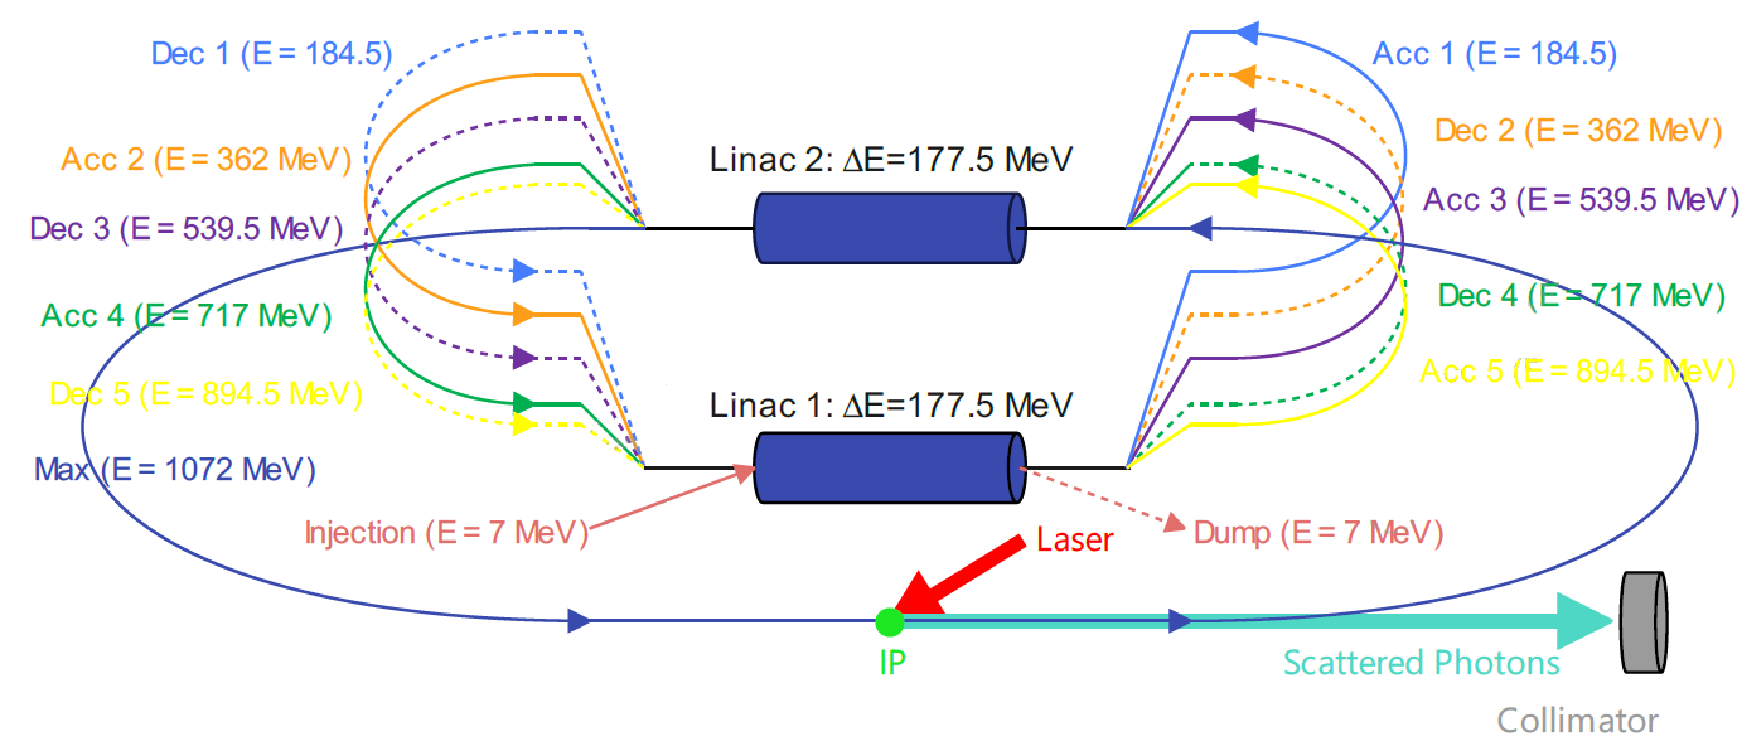
\includegraphics[width=0.9\textwidth]{Figures/DIANA_Inverse_Compton_Source_Design/DIANA_diagram_fixed.pdf}
\caption{Drawing of the 3-turn DIANA ERL, utilising dual symmetric linacs (dark blue) and separate transport -- where each accelerating (solid line) and decelerating (dashed line) pass is transported in a separate beamline. A total of 6 different energies, noted on the diagram, will be transported by the DIANA ERL. A possible schematic for an ICS source is presented, with an IP (green), where the counter-propagating laser (red) interacts with the electron bunch (blue) to scatter photons (turquoise) and is collimated downstream (grey).}
\label{fig:DIANA_ERL_diagram}
\end{figure}
Within the context of the wider particle accelerator landscape, DIANA would be a national scale facility and is aligned to two projects in particular: a proposal for the UK-XFEL \cite{burnett2020uk} and as a solution for the Large Hadron--electron Collider (LHeC) \cite{valloni2013strawman,bruning2019exploring,holzer2021accelerator,agostini2021large}. A partial ERL solution with an ICS source is one of three suggested accelerator solutions to a UK x-ray free electron laser presented in the UK-XFEL science case \cite{burnett2020uk}. The UK-XFEL ICS source design is a precursor to the DIANA ICS source design, as a UK-XFEL ICS source could be a potential demonstrator for the DIANA ERL. The DIANA ERL could also act as a proof-of-principle for the LHeC ERL alongside the PERLE accelerator \cite{angal2018perle}, demonstrating another design and transport approach.

High brilliance electron beams on the \si{\giga\electronvolt} scale can facilitate applications such as a high-power extreme ultraviolet (EUV) FEL \cite{akkermans2017compact} and a $\gamma$-ray inverse Compton scattering source \cite{hajima2008proposal,hajima2014application}. Tunability of the electron bunch energy of the ERL is necessary for many light source experiments and must be central to the design philosophy of DIANA for useful operation of the ICS source and EUV FEL. 

In photo-lithography high average powers of UV radiation $\lambda=193$~\si{\nano\meter} (the current industry standard wavelength \cite{socol2011compact}) are required to nanopattern silicon wafers for the production of integrated circuits. However, wavelengths below 193~\si{\nano\meter} are necessary for further miniaturisation of integrated circuitry to keep pace with Moore's law; every two
years the density of chip transistors is doubled \cite{moore1975international}. Wavelengths of 13.5~\si{\nano\meter} are targeted because these offer nanopatterning to within a 10~\si{\nano\meter} resolution \cite{wagner2010lithography} however, only two technologies have been identified for high average power EUV production: laser produced plasma sources, such as the ASML NXE:3100 \cite{wagner2011euv,socol2011compact}, and EUV FELs \cite{socol2011compact,akkermans2017compact}. FELs may offer a higher average power EUV source of around 5~\si{\kilo\watt} average EUV power \cite{akkermans2017compact} whereas laser produced plasma sources have demonstrated up to 125~\si{\watt} \cite{} -- a factor $\sim5$ increase in power and consequently an increased production rate. In summary, an EUV FEL source would have far-reaching consequences for semiconductor lithography providing an unparalleled source of 13.5~\si{\nano\meter} EUV radiation (or some harmonic thereof) \cite{socol2011compact}.  

A high flux, narrowband $\gamma$-ray inverse Compton scattering source driven by the DIANA ERL is another possible application. ERL driven $\gamma$-ray ICS sources would have considerable impact upon nuclear physics and security \cite{budker2021expanding} by reducing the bandwidth of the produced $\gamma$-rays which limits experiments currently performed at world-leading storage ring driven $\gamma$-ray ICS source facilities such as HI$\gamma$S \cite{weller2009research}. HI$\gamma$S is currently the highest energy $E_{\gamma} \sim 100$~\si{\mega\electronvolt} and highest flux $\mathcal{F} \sim 10^{9}$~ph/\si{\second} $\gamma$-ray source but is limited to a $\sim2$\% FWHM bandwidth \cite{weller2009research}.  The focus of this thesis is on the development of the DIANA $\gamma$-ray ICS source and its applications, as well a progress toward a conceptual design of the DIANA ERL, hence the following chapter excludes EUV FEL developments.

A $\gamma$-ray ICS source at moderate energies ($E_{\gamma} < 5$~\si{\mega\electronvolt}) could enable applications such as nuclear resonance fluorescence (NRF) for inspection of nuclear fuel rods, waste studies and detection of clandestine nuclear material \cite{angell2015demonstration,bolind2015states} whereas higher energy ($E_{\gamma} > 5$~\si{\mega\electronvolt}) allows applications such as nuclear photonics \cite{budker2021expanding} and medical isotope production \cite{habs2011production}, as explained in Section~\ref{sec:DIANA_ICS_applications}. The scattered photon energy regime of nuclear photonics lies in the $\sim$20~\si{\mega\electronvolt} regime and above; therefore the electron bunch energy of the DIANA ERL must enable $\gamma$-ray production in this range. However, the scattered photon energy of the DIANA ICS source could also be doubled ($E_{\gamma}\sim 40$~\si{\mega\electronvolt}) through use of frequency doubled lasers (see Section~\ref{sec:lasers_fabry_perot}), such as the commonly used 2nd harmonic of a Nd:YAG ($\lambda =$532~\si{\nano\meter}) laser. A range of applications are investigated in Section~\ref{sec:DIANA_ICS_applications} with greater consideration given to the photo-nuclear production of medical isotopes. 

\begin{figure}[!h]
\centering
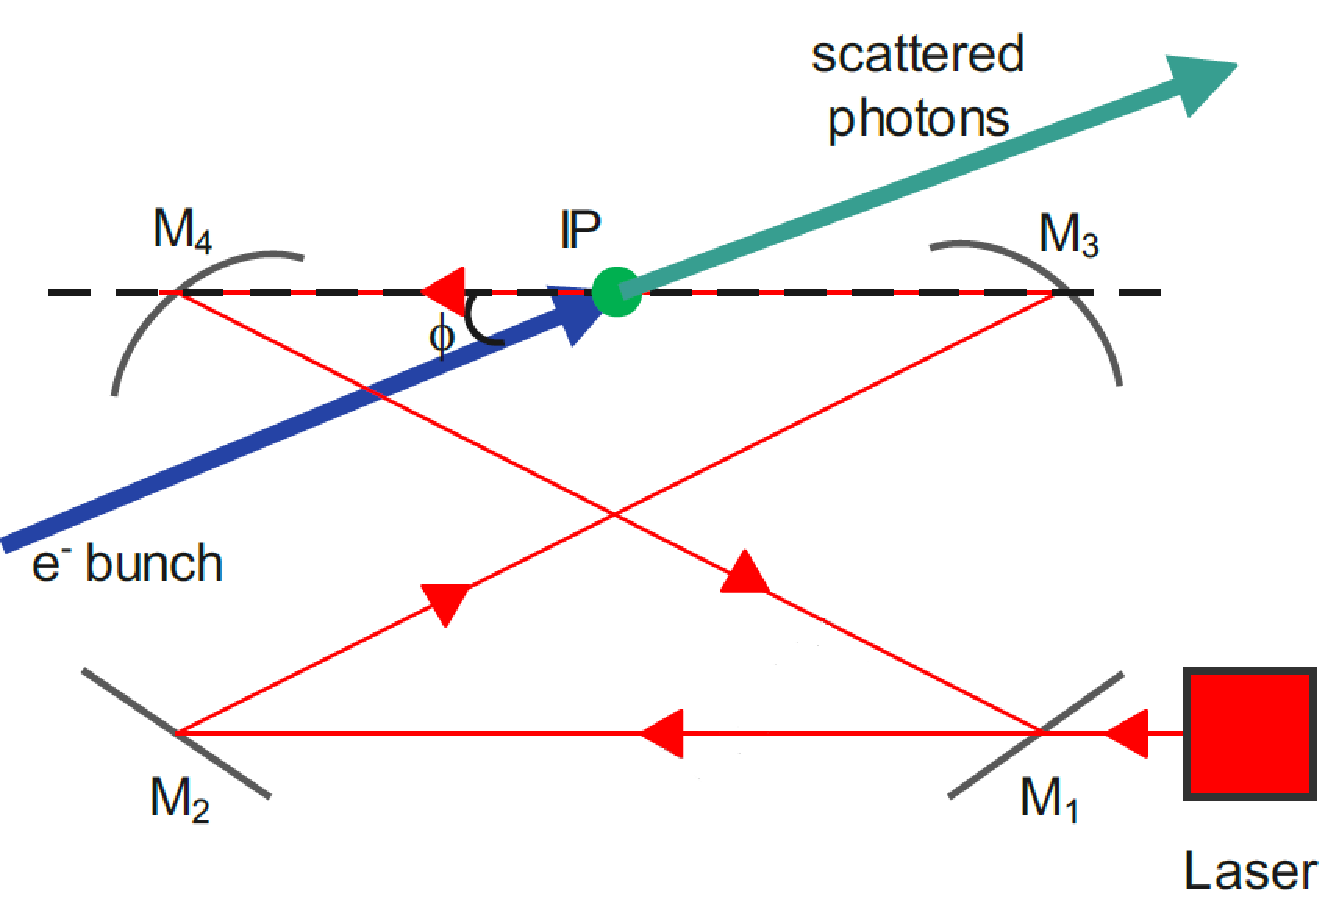
\includegraphics[width=0.6\textwidth]{Figures/DIANA_Inverse_Compton_Source_Design/DIANA_interaction_fixed.pdf}
\caption{Interaction of an electron bunch (blue) with an Nd:YAG laser ($\lambda = 1064$~\si{\nano\meter}) pulse (red) at a crossing angle $\phi=5$\si{\degree} at the IP (green) placed at the centre of the electron bunch final focus system. Photons are scattered (turquoise) in a similar direction to the incident electron bunch. The laser pulse is re-circulated many times in the 4-mirror (grey) Fabry-Perot optical cavity.    }
\label{fig:DIANA_interaction}
\end{figure}
The designed DIANA ICS source will utilise the electron bunch provided by the ERL at interaction points integrated directly into the transport optics, unlike the bypass design for the CBETA ICS in Chapter~\ref{CBETA_Inverse_Compton_Scattering_Source_Design}, to produce a multi-colour $\gamma$-ray source taking advantage of three nominal electron bunch energies of the DIANA ERL (resulting from the three turns, $E_{e}=$362, 717, 1072~\si{\mega\electronvolt}). A high average power 4-mirror Fabry-Perot optical re-circulation cavity is proposed to store a Nd:YAG laser pulse ($\lambda = 1064$~\si{\nano\meter}) and interact the laser pulses with the electron bunches at a high repetition rate, producing a high flux of $\gamma$-rays and taking advantage of the re-circulated electron bunch in an ERL; a schematic of the ICS interaction is shown in Fig.~\ref{fig:DIANA_interaction}. As shown in Fig.~\ref{fig:DIANA_ERL_diagram}, A variable aperture circular collimator placed 10~\si{\meter} from the interaction point will then select the monochromatic $\gamma$-rays for narrowband operation (at the users bandwidth specification); taking advantage of the energy--angle correspondence (see Section~\ref{sec:derivation_of_the_scattered_photon_energy}). Within this chapter the DIANA ERL is outlined and the design of the ICS interaction points, using optimisation procedures developed in Chapter~\ref{Optimisation_and_Characterisation_of_Inverse_Compton Scattering_Spectra}, is presented for narrowband ($< 1$\% \textit{rms}) $\gamma$-ray production on the \si{\mega\electronvolt}-scale. 

\section{The Conceptual DIANA ERL Design}
\label{sec:DIANA_ERL_design}

The conceptual DIANA ERL is a 3 turn (6 pass) electron energy recovery linac with dual SRF linacs (12 linac passes) in a racetrack topology, designed for light source operation ($\gamma$-ray ICS source and EUV FEL). A maximum electron bunch energy of 1072~\si{\mega\electronvolt} is proposed. The DIANA ERL is designed to be CW, with an average beam current of 12.5~\si{\milli\ampere} delivering 100~\si{\pico\coulomb} electron bunches at a bunch repetition rate of 125~\si{\mega\hertz}. The design aims for a high electron brightness -- high average beam current with a small emittance ($\epsilon_{n}=0.5$~\si{\milli\meter}--\si{\milli\radian}) -- and a small energy spread ($\Delta E_{e}/E_{e} \sim 10^{-5}$), crucial for high brilliance light sources. Parameters of the DIANA ERL are shown in Table~\ref{tab:GeV_ERL_design_parameters}, and expanded upon for the $\gamma$-ray ICS source in Table~\ref{tab:DIANA_electron_beam_design_parameters} with a detailed explanation of the design parameters presented in Section~\ref{sec:DIANA_electron_parameters}. Discussions in this section focus on ERL design concepts and contextualising the DIANA ERL, not the justification of ERL parameters. 

Design of the DIANA energy recovery linac is an ongoing project. Two of the most critical design choices -- the choice of dual linacs and single transport -- are discussed here, with reference to the development of DIANA as a light source facility and with focus on the proposed multi-colour ICS source. Therefore, the following sections present the design choices with reference to other similar \si{\giga\electronvolt}-scale ERL projects: the PERLE ERL \cite{angal2018perle}, the ER@CEBAF multi-turn ERL \cite{meot2016er} and the ERL FEL design by Akkermans et al \cite{akkermans2017compact}. Parameters of these ERL designs and the proposed DIANA ERL design are shown in Table~\ref{tab:GeV_ERL_design_parameters}.

\begin{table}[!h]
\centering
\caption{Parameters of some proposed multi-turn \si{\giga\electronvolt}-scale energy recovery linac projects around the world. ERLs such as the DIANA ERL and EUV-FEL ERL are designed for light source operation whereas the CEBAF and PERLE ERLs are designed as demonstrators for future particle collider or fundamental nuclear physics experiments.}
\vspace{3mm}
\begin{threeparttable}
\resizebox{\columnwidth}{!}{
\begin{tabular}{lccccc}
\hline\hline
Parameter & ER@CEBAF \cite{meot2016er,bogacz2016er} & PERLE \cite{angal2018perle,kaabi2019perle} & EUV-FEL ERL \cite{akkermans2017compact} & DIANA & Unit \\
\hline
No. Turns & 5 & 3 & 2 & 3 &   \\
Injection Energy, $E_{\mathrm{inj}}$ & 79 & 7 & 9.91 & 7 & \si{\mega\electronvolt}\\
Max Electron kinetic energy, $E_e$ & 7080 & 487 & 748 & 1072 & \si{\mega\electronvolt}\\
Bunch charge, $e N_e$ & 0.2 & 500 & 70 & 100 & \si{\pico\coulomb} \\
Average beam current, $I$ & 0.1 & 20 & 45.5 & 12.5 & \si{\milli\ampere} \\
Trans. norm. \textit{rms} emittance, $\epsilon_{N}$ & 3~\tnote{*} & 6 & 0.4 & 0.5 & \si{\milli\meter}-\si{\milli\radian}\\
\textit{rms} bunch length, $\Delta\tau$ & 0.09--0.12 (0.3--0.5) & 3 (10) & 0.9 (3) & 0.9 (3) & \si{\milli\meter} (\si{\pico\second})\\
Bunch frequency, $f_{\mathrm{bunch}}$ & 249.37 & 40 & 649.35 & 125 & \si{\mega\hertz} \\
RF frequency, $f_{RF}$ & 1497 & 801.58 & 650 & 750 & \si{\mega\hertz} \\
Rel. energy spread, $\left(\Delta E_{e}/E_{e}\right)$ & 0.02-0.03 & - & $3\times 10^{-4}$ &  $\sim5\times 10^{-5}$ & \\
\hline\hline
\end{tabular}}
\begin{tablenotes}
\item[*]{The normalised emittance at injection into CEBAF is $\epsilon_{n} = 1.56$~\si{\milli\meter}-\si{\milli\radian}, however the}
\item{design parameter of Meot et al \cite{meot2016er} is used here.}
\end{tablenotes}
\end{threeparttable}
\label{tab:GeV_ERL_design_parameters}
\end{table}

\subsection{Dual Linacs}

The DIANA design proposes dual symmetric SRF linacs which are incorporated into the ERL racetrack, as shown in Fig.~\ref{fig:DIANA_ERL_diagram}. Using dual linacs in the racetrack layout minimises the footprint of the accelerator in comparison to a single linac design, such as the CBETA ERL in Chapter~\ref{CBETA_Multi-Pass_Commissioning}, as the required acceleration section length can be halved. Energy recovery linacs such as PERLE \cite{angal2018perle} and CEBAF \cite{meot2016er} achieve high energies in a layout more compact than a single linac design primarily because of the dual linac racetrack. However, an extra two spreader sections are required to re-combine the 3-turns (6-passes) of DIANA into a single beamline for on-axis traversal of the second linac, then to re-split the beamlines back into the 6 different passes after the linac traversal. Using symmetric linacs (see Section~\ref{sec:dual_linac_ERL}) would mean that the electron bunch energies transported in the beamlines are spaced by equal successive intervals; with an energy gain per turn of 355~\si{\mega\electronvolt}, the beamlines after each linac pass differ by 177.5~\si{\mega\electronvolt}. The regular electron beam energy intervals between passes may mean that spreader design is more simplistic; however, an asymmetric solution may be easier to implement -- this aspect requires further study. In addition, with 6 passes -- required by separate transport (see Section~\ref{sec:ERL_transport_options}) -- the spreader sections would be spatially complex with many nearby magnets and may experience cross-talk -- where magnetic fields overlap -- which would be difficult to design and implement. Multi-turn separate transport spreaders have not been demonstrated in design studies with a dual linac approach, as both CEBAF \cite{meot2016er} and PERLE \cite{angal2018perle} are common transport ERLs, therefore design of this section of the DIANA ERL may prove challenging. 

Utilising dual symmetric linacs would mean a total of 6 different electron energies would be present in the DIANA ERL (i.e each turn/beampipe contains two electron energies). The additional electron energies are available to a potential light source operating on the ERL, therefore this could provide a simple route to a multi-colour $\gamma$-ray source if an ICS source interaction point is placed after each linac pass. Fully integrated interaction points within the DIANA design would avoid the necessity of complex bypass designs like those for the CBETA ICS source in Section~\ref{sec:bypass_design}. However, with more electron energies transported in the ERL the transport optics must be designed to transport more electron beam energies, and are therefore more complicated. To the authors knowledge, dual linac multi-turn ERLs have not been proposed for light source operations but may provide tuneable sources of electrons at a variety of electron energies within a compact footprint that may be ideal for a multi-colour light source.

\subsection{Separate Transport}

The separate transport approach to multi-turn ERLs -- where each accelerating and decelerating configuration of the electron bunch, at each nominal electron energy, is transported in a separate beamline (see Section~\ref{sec:ERL_transport_options}) -- has been utilised previously in the ERL FEL design by Akkermans et al \cite{akkermans2017compact}. Therefore, single transport is a more established option for ERL based light sources, such as the DIANA proposal, than common transport approaches which have not demonstrated light source operation. Single transport may be particularly useful for ERL driven ICS sources as each beamline transports a single electron bunch configuration (accelerating or decelerating) at a single energy. Therefore, varying the optics of a single beamline in a single transport ERL does not vary optics of other beamlines, as long as the electron bunch at the entrance to the linac for the next pass remains unchanged. Consequently, interaction points with variable focusing -- as needed to provide narrowband optimised radiation production (see Chapter~\ref{Optimisation_and_Characterisation_of_Inverse_Compton Scattering_Spectra}) -- can be integrated into this design more easily because there are less optics constraints than from multiple electron energy transport optics.

In comparison, for a common transport ERL an ICS interaction point would have to focus both electron bunches on the accelerating and decelerating passes to the same electron bunch spot size at the interaction point and, as the produced spectrum of scattered photons is sensitive to the electron bunch distribution, the bunch would have to be in an identical configuration. If these conditions weren't obeyed the ICS spectral output to a user would be variable. Separate transport is consequently a more simple transport option for a multi-turn ERL light source. However, single transport ERLs typically use more magnets and beamline infrastructure which adds to the expense of an ERL project. In summary, the separate transport approach to an ERL light source may provide advantages of easier integration of ICS sources and more reproducible scattered photon production at the cost of a greater number of accelerator magnets.  

\section{ERL ICS Electron Beam and Optical Cavity Laser Pulse Parameters}

\subsection{ERL ICS Electron Beam Parameters }
\label{sec:DIANA_electron_parameters}

The proposed electron bunch parameters for the DIANA ERL ICS source are presented in Table~\ref{tab:DIANA_electron_beam_design_parameters}. The proposed parameters are broadly applicable to development of a high brilliance FEL though an EUV FEL would require some adjustment to the longitudinal parameters as coherence in FELs demands short bunch lengths and high peak electron beam powers. The ERL ICS source parameters for the ICS source would be tunable to the requirements of an EUV FEL. 

Baseline electron bunch parameters are proposed to characterise the bare, uncollimated spectrum of the $\gamma$-ray radiation produced by the DIANA ICS source when the ICS source is configured solely for high flux operation, not for narrow bandwidth. High flux operation of an ICS $\gamma$-ray source requires small electron bunch spot sizes, therefore a small $\beta$-function at the IP in the baseline design case is specified ($\beta^{*}=0.2$~\si{\meter}). Round beams at the IP for the baseline case are chosen for simplicity, and because a round bunch is a decent approximation to electron bunches in ERLs. Constant $\beta$-functions in the baseline case allow the effect of electron bunch energy variation in each turn to be inspected. The $\gamma$-ray production from an ICS source is quantified by performance parameters such as the uncollimated flux (Eq.~\ref{eq:flux_angular_crossing_hourglass}), spectral density (Eq.~\ref{eq:spectral_density}), average (Eq.~\ref{eq:average_brilliance}) and peak (Eq.~\ref{eq:peak_brilliance}) brilliance, as calculated in Table~\ref{tab:DIANA_spectral_output} for the DIANA ICS. The performance parameters can be satisfactorily calculated for an uncollimated ICS source and are consequently limited to the baseline case here. Because ICS sources, and light sources more generally, are compared via these performance parameters the baseline case enables comparison between the proposed DIANA ICS source design and other projects, as shown in Section~\ref{sec:gamma_ICS_comparison}, which may not be designed toward the narrowband radiation production goals of DIANA.

The electron bunch parameters have also been optimised for narrowband operation ($\left(\Delta E_{\gamma}<1\%\right)$) of the ICS source using the simplex non-round beam optimisation described in Section~\ref{sec:NRB_optimisation}, as this optimisation produced the highest collimated flux within the specified bandwidth of the source ($\Delta E_{\gamma}/E_{\gamma}=0.5\%$, \textit{rms}). Narrowband optimisation provides insight on the ability of the DIANA ICS source design to provide the quasi-monochromatic radiation most favoured by users for high precision nuclear physics experiments. Single point optimisations (see Section~\ref{sec:objective_functions_and_variables}) -- optimisations for a single bandwidth value --  are specified for a narrowband 0.5\% \textit{rms} bandwidth, chosen because a \textit{rms} 0.5\% bandwidth is comparable to the state-of-art ELI-NP-GBS \cite{elinp2019vega} $\gamma$-ray ICS source. Tuning curve optimisations shown later in this section (in Figs.~\ref{fig:DIANA362_param}, \ref{fig:DIANA717_param}, \ref{fig:DIANA1072_param}), with solution space results in Section~\ref{sec:DIANA_spectral_output}, are performed across the narrowband range (0--1\% \textit{rms} bandwidth).    
\begin{table}[!h]
\centering
\caption{Electron beam parameters foreseen at the DIANA ICS source interaction point (IP). Baseline parameters assume a round transverse profile for the electron bunch whereas the optimised parameters are the result of simplex non-round beam optimisation. The given baseline parameters -- which assume the same $\beta^*$ at the IP -- allow a comparison of flux and bandwidth at different energies. The optimised values beneath those are designed to maximise the flux into a 0.5\% \textit{rms} scattered photon bandwidth through a trade-off of $\beta$-function of the electron bunch in each transverse plane and collimation angle.}
\vspace{3mm}
\begin{threeparttable}
\resizebox{\columnwidth}{!}{
\begin{tabular}{lccccc}
\hline\hline
Parameter & \multicolumn{3}{c}{Quantity} & Unit \\
\hline
Turn number & 1 & 2 & 3  \\
Injection Energy, $E_{\mathrm{inj}}$ & \multicolumn{3}{c}{7} & \si{\mega\electronvolt}\\
\tnote{$\dagger$}~Electron kinetic energy, $E_e$ & 362 & 717 & 1072 & \si{\mega\electronvolt}\\
Harmonic Frequency, $f$ & \multicolumn{3}{c}{125} & \si{\mega\hertz}\\
Bunch charge, $e N_e$ & \multicolumn{3}{c}{100} & \si{\pico\coulomb} \\
Average beam current, $I$ & \multicolumn{3}{c}{12.5} & \si{\milli\ampere} \\
Transverse normalised \textit{rms} emittance, $\epsilon_{N}$ & \multicolumn{3}{c}{0.5} & \si{\milli\meter}-\si{\milli\radian}\\
\tnote{$\sharp$}~\textit{rms} bunch length, $\Delta \tau$ & \multicolumn{3}{c}{0.9 (3)} & \si{\milli\meter} (\si{\pico\second})\\
Bunch spacing, $t_{b}$ & \multicolumn{3}{c}{8} & \si{\nano\second} \\
RF frequency, $f_{RF}$ & \multicolumn{3}{c}{750} & \si{\mega\hertz} \\
\tnote{*}~Absolute energy spread, $\Delta E_{e}$ & \multicolumn{3}{c}{$\sim$10--50} & \si{\kilo\electronvolt} \\ 
\tnote{*}~Relative energy spread, $\left(\Delta E_{e}/E_{e}\right)$ & \multicolumn{3}{c}{$\sim5\times 10^{-5}$} & \\
\hline
\multicolumn{5}{c}{Baseline Parameters} \\
\hline
$\beta$-functions at the IP, $\beta_{x}^{*}$/$\beta_{y}^{*}$ & 0.2/0.2 & 0.2/0.2 & 0.2/0.2 & \si{\meter} \\
Electron bunch spot size, $\sigma_{e,x}$/$\sigma_{e,y}$ & 11.87/11.87 & 8.44/8.44 & 6.90/6.90 & \si{\micro\meter}\\
\hline\multicolumn{5}{c}{Optimised 0.5\% \textit{rms} Bandwidth} \\
\hline
$\beta$-functions at the IP $\beta_{x}^{*}$/$\beta_{y}^{*}$ & 1.33/0.298 & 2.62/0.587 & 3.90/0.874 & \si{\meter} \\
Electron bunch spot size, $\sigma_{e,x}$/$\sigma_{e,y}$ & 30.62/14.49 & 30.54/14.46 & 30.48/14.43 & \si{\micro\meter}\\
Collimation Angle, $\theta_{\mathrm{col}}$ & 0.180 & 0.091 & 0.061 & \si{\milli\radian} \\ 
\hline\hline
\end{tabular}}
\begin{tablenotes}
\item[$\sharp$]{Based on the ASML FEL parameters \cite{akkermans2017compact}}
\item[*]{Estimated values.}
\item[$\dagger$]{Electron beam energies to accomplish $E_{\gamma}^{\mathrm{max}}$ = 20~\si{\mega\electronvolt} $\gamma$-rays.}
\item{Electron energy variation per turn $\Delta E_{\mathrm{turn}} =$ 355~\si{\mega\electronvolt}.}
\end{tablenotes}
\end{threeparttable}
\label{tab:DIANA_electron_beam_design_parameters}
\end{table}

% electron bunch energy
The nominal electron kinetic energies of the DIANA 3 turn ERL are 362, 717, 1072~\si{\mega\electronvolt} with a difference in energy per turn of 355~\si{\mega\electronvolt} due to acceleration or deceleration in the dual linacs; injection is at 7~\si{\mega\electronvolt}. A 7~\si{\mega\electronvolt} injection energy is identical to the PERLE \cite{angal2018perle} ERL injection energy and similar to demonstrated multi-turn ERL projects such as CBETA ($E_{\mathrm{inj}}=6$~\si{\mega\electronvolt}) \cite{bartnik2020cbeta} and S-DALINAC ($E_{\mathrm{inj}}=7.6$~\si{\mega\electronvolt}) \cite{arnold2018first}. \si{\mega\electronvolt}-scale injection energies are relativistic and above transition, which simplifies the longitudinal beam dynamics within an ERL (see Chapter~\ref{Energy_Recovery_Linac_Design}). Modern photo-injectors also operate at high average beam current within the 5--10~\si{\mega\electronvolt} electron energy range, such as the world-leading Cornell photoinjector \cite{bartnik2015operational}. 

A maximum electron energy of 1072~\si{\mega\electronvolt} is selected as -- with a Nd:YAG laser ($\lambda=1064$~\si{\nano\meter}) -- this allows production of 20~\si{\mega\electronvolt} $\gamma$-rays. A 1072~\si{\mega\electronvolt} maximum energy also reflects the limitations imposed upon the ERL by both physical size and coherent synchrotron radiation losses. For example, assuming a 20~\si{\mega\volt}/\si{\meter} accelerating electric field \cite{ben2006review}, symmetric linacs and an 80\% filling factor (the same as CBETA \cite{hoffstaetter2017cbeta}) $\sim$11~\si{\meter} long linacs are required, and an accelerator circumference of $\sim$100's~\si{\meter} is expected (subject to full design study). The nominal energies of the previous turns are fixed at 362~\si{\mega\electronvolt} and 717~\si{\mega\electronvolt} due to the 355~\si{\mega\electronvolt} energy gain per turn. However, the first turn electron energy ($E_{e}=362$~\si{\mega\electronvolt}) is advantageous because scattered photon energies around the 1.5--3~\si{\mega\electronvolt} phton energy range for nuclear resonance fluorescence experiments \cite{angell2015demonstration,quiter2011transmission} can be produced. 

% RF Frequency + electron bunch frequency
An RF frequency of 750~\si{\mega\hertz} is proposed because this is typical of state-of-the-art SRF developments within SRF technologies, where stable CW acceleration is available in the 600--800~\si{\mega\hertz} range \cite{calaga2013proposal}, and studies for the LHeC ERL configuration have proposed similar RF frequencies ($f_{\mathhrm{RF}}=802.5$~\si{\mega\hertz}) \cite{agostini2021large}. For example, a Jefferson Laboratory prototype single cell SRF cavity has achieved accelerating gradient of $E_{\mathrm{acc}}=25$~\si{\mega\volt}/\si{\meter} at a 748.5~\si{\mega\hertz} RF frequency \cite{rimmer2007jlab}, which would satisfy the DIANA ERL design parameters. 

% maximum possible is 1/6?
The proposed bunch repetition frequency of DIANA is 125~\si{\mega\hertz}, 1/6th of the RF frequency because DIANA is a CW ERL with a total of 6 linac passes and 6 simultaneously circulating electron bunches. The electron bunch repetition rate is also fixed by the requirement that the laser pulse and electron bunch must interact at the same rate, therefore the Fabry-Perot optical cavity must have an identical repetition frequency (or some harmonic thereof) for interaction of each electron bunch with a laser pulse. The ideal repetition frequency of both systems is 125~\si{\mega\hertz} (a path length of 2.4~\si{\meter}) because of the laser pulse optical re-circulation cavity limitations mentioned in Section~\ref{sec:DIANA_laser_fabry_perot}.

% Beam Current (Bunch Charge and REP FREQ dependence) + emittance
Modern photo-injectors are capable of delivering bunch charges into the 100's~\si{\pico\coulomb} range \cite{angal2018perle,hounsell2021optimization} -- for example the Cornell photoinjector demonstrated a 100~\si{\pico\coulomb} electron bunch with a transverse emittance of $\epsilon_{nx}~\left(\epsilon_{ny}\right) = 0.37~ (0.39)$~\si{\milli\meter}--\si{\milli\radian} \cite{bartnik2015operational}. Consequently, a 100~\si{\pico\coulomb} bunch charge is selected for DIANA which, with a 125~\si{\mega\hertz} bunch repetition frequency, corresponds to a 12.5~\si{\milli\ampere} average beam current. A small transverse emittance of $\epsilon_{n}=0.5$~\si{\milli\meter}--\si{\milli\radian} is also proposed for the DIANA ERL because this is well within the state-of-the-art of the demonstrated Cornell photoinjector.

A previous design study for an EUV FEL using a 750~\si{\mega\electronvolt} multi-turn electron ERL with a 100~\si{\pico\coulomb} bunch charge and similar transverse normalised emittance by Akkermans et al\cite{akkermans2017compact} shows that transport of the DIANA bunch charge and small normalised emittance is feasible. Bunch charges in ERLs on the 10's~\si{\pico\coulomb}-scale have been demonstrated, such as the J-Lab FEL, where energy recovery with 60~\si{\pico\coulomb} electron bunches \cite{benson1999first} was achieved. The average power of the DIANA electron beam is 13.4~\si{\mega\watt}, a factor of 2.23 larger than the electron beam power in the CBETA ERL proposal as described in Chapter~\ref{CBETA_Multi-Pass_Commissioning}, and similar to the PERLE proposal \cite{angal2018perle}. However, average current is limited by collective effects such as coherent synchrotron radiation (CSR) and beam break-up (BBU) instabilities arising during transport in the ERL. Beam break-up studies for the CBETA ERL have demonstrated that an average beam current threshold of up to 40~\si{\milli\ampere} is possible within the CBETA ERL \cite{lou2019beam} and similarly a 10's~\si{\milli\ampere} threshold would be expected for DIANA. An increase in coherent synchrotron radiation production is expected for DIANA relative to CBETA because the bunch charge (number of electrons) is larger which increases the CSR power emitted ($P_{\mathrm{CSR}} \propto N_{e}^{2}$) and the electron beam energy is larger ($1072~\mathrm{\si{\mega\electronvolt}} > 150~\mathrm{\si{\mega\electronvolt}}$) causing a large increase in emitted power ($P_{\mathrm{CSR}}\propto \gamma^{4}$). Therefore, more in depth studies -- beyond the scope of this thesis -- are required to validate the proposed parameters. 

% Bunch length
Short \textit{rms} bunch lengths (durations) of $\sigma_{z}=0.9$~\si{\milli\meter} (3~\si{\pico\second}) predicted for DIANA are based upon the ERL EUV FEL design by Akkermans et al\cite{akkermans2017compact} because of similarities in the separate transport design for DIANA. However, a short electron bunch duration is only desirable for an ICS source interaction if the time duration of the radiation is critical for applications. This is dissimilar to FEL operation where a short bunch length is required for coherence and a high peak beam current. The scattered photon duration of ICS sources also depends on the laser pulse duration, so electron bunch lengths much shorter than the laser pulse duration in the Fabry-Perot optical cavity are not beneficial. A 3~\si{\pico\second} electron bunch duration is of similar scale to the 10's~\si{\pico\second} pulse durations demonstrated in Fabry-Perot optical cavities and a short bunch duration ensures minimal geometric luminosity reduction, because the reduction in laser pulse--electron bunch overlap in the interaction is not substantially reduced (see Section~\ref{sec:geometric_luminosity_reduction}).  . 

% Bunch Energy Spread
A small electron bunch energy spread is necessary for the production of narrowband radiation from an ICS source. The bandwidth of an ICS source is directly proportional to the energy spread of the electron bunch (Eq.~\ref{eq:RMS_bandwidth}), therefore it is necessary to minimise the energy spread of the electron bunch for light source operations. The electron bunch energy spread proposed for DIANA in Table~\ref{tab:DIANA_electron_beam_design_parameters} ($\Delta E_{e} \sim 10$~\si{\kilo\electronvolt}) is based upon the 6~\si{\kilo\electronvolt} uncorrelated electron energy spread that is readily demonstrated at the EuXFEL \cite{tomin2021accurate} for a 250~\si{\pico\coulomb} electron bunch. 

% Optimisations
The three DIANA ICS sources at each turn energy ($E_{e}=$362, 717, 1072~\si{\mega\electronvolt}) have been optimised for a 0.5\% \textit{rms} bandwidth using the three optimisation methods (RB, simplex NRB and GA NRB) outlined in Chapter~\ref{Optimisation_and_Characterisation_of_Inverse_Compton Scattering_Spectra}. The optimised electron beam interaction parameters and collimation parameters resulting from the single point 0.5\% \textit{rms} bandwidth optimisations are shown in Table~\ref{tab:DIANA_electron_beam_design_parameters}, which provide a snapshot of a potential DIANA ICS source in a narrowband configuration. However, the focus here is on the parameter space (collimation angle $\theta_{\mathrm{col}}$ and $\beta_{x/y}$-functions in each plane) tuning curve optimisations in the narrowband range ($0 \leq \Delta E_{\gamma}/E_{\gamma} \leq 1$\% \textit{rms} bandwidth) used to map the tunability required in the electron bunch final focus and $\gamma$-ray collimation systems. Laser pulse parameters remain unchanged from Table~\ref{tab:DIANA_laser_pulse_design_parameters}. Parameter space tuning curves are produced for each of the three nominal electron energies of the DIANA ERL, as shown in Figs.~\ref{fig:DIANA362_param}, \ref{fig:DIANA717_param}, \ref{fig:DIANA1072_param}. Parameter space tuning curves correspond to the Pareto front points in the collimated flux--\textit{rms} bandwidth solution space in Fig.~\ref{fig:DIANAFBW}, shown in Section~\ref{sec:DIANA_spectral_output}.
\begin{figure}[!h]
\centering
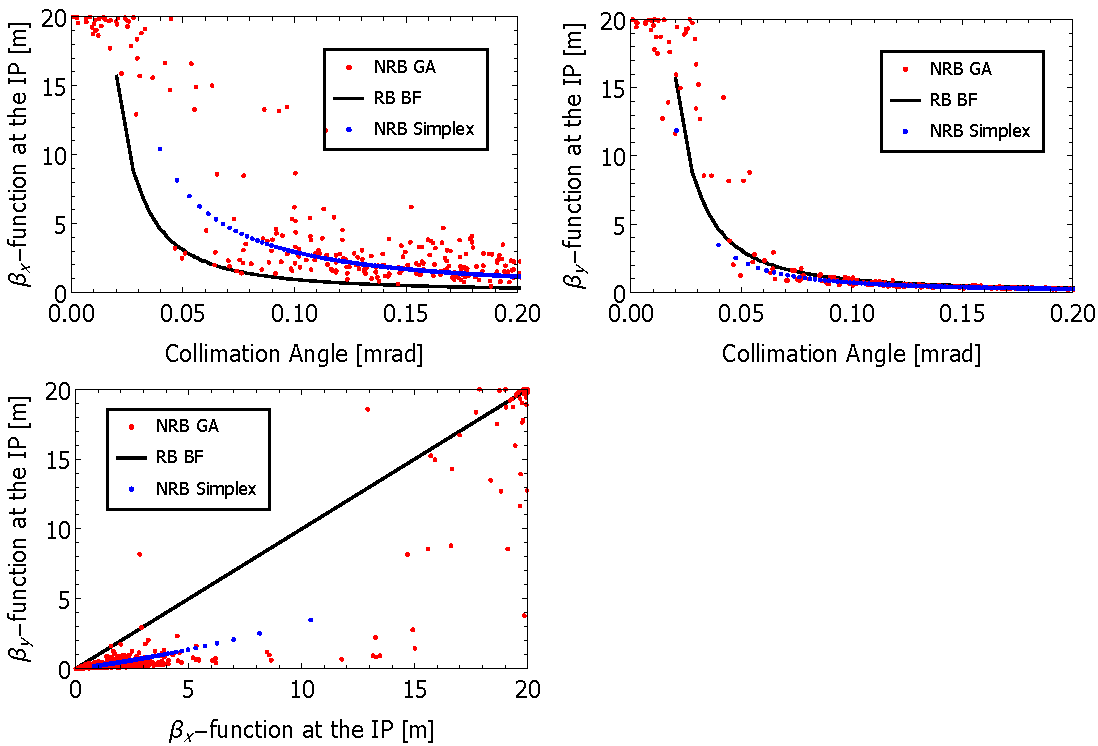
\includegraphics[width=\textwidth]{Figures/DIANA_Inverse_Compton_Source_Design/DIANA362param.pdf}
\caption{DIANA 362~\si{\mega\electronvolt} 1st turn ICS source optimisations, comparing the two non-round beam approaches (simplex (blue) and GA (red)) and the round beam approach (black). Top Left: parameter space of the interaction $\beta$-function in the $x$ plane and collimation angle for optimised cases. Top Right: parameter space of the interaction $\beta$-function in the $y$ plane and collimation angle for optimised cases.  Bottom Left: interaction point $\beta$-function parameter space in the $x$ and $y$ plane for optimised cases. Elliptical electron bunches are favoured at the IP, with a larger horizontal beam size because of the laser pulse--electron bunch crossing angle in the horizontal $X$ plane.}
\label{fig:DIANA362_param}
\end{figure}

The top plots of parameter space tuning curves of the DIANA ICS source at an electron bunch energy of $E_{e}=362$~\si{\mega\electronvolt} in Fig~\ref{fig:DIANA362_param} show the $\beta$-functions at the IP in each plane against the required collimation angle, for each of the three optimisation methods under consideration. The $\beta_{x}^{*}$--$\theta_{\mathrm{col}}$ plot shows that the non-round beam optimisations maintain the same shape as evident in the non-round beam cases in Section~\ref{sec:RB_optimisation}. However, the simplex and GA tuning curves are offset from the round beam tuning curve because of the non-zero crossing angle and the gradient of the Pareto front is less severe because the $\beta_{x}^{*}$-functions are increased to increase the overlap of the electron bunch and laser pulse. The small collimation angle (large $\beta^{*}$-function) end of the Pareto front typically relates to the narrowest bandwidth portion of the tuning curve whereas the large collimation angle (small $\beta^{*}$-function) solutions relate to larger bandwidths in the range. Maximising collimation angle and minimising $\beta$-functions in each plane is optimal for collimated flux (Eq.~\ref{eq:collimated_flux}) but these must be kept small for narrow bandwidth which is limited by the emittance (Eq.~\ref{eq:emittance_term}) and collimation (Eq.~\ref{eq:collimation_term}) terms of the bandwidth (Eq.~\ref{eq:RMS_bandwidth}). The genetic algorithm $\beta_{x}^{*}$--$\theta_{\mathrm{col}}$ parameter space Pareto optimal points are spread in this plot highlighting the insensitivity of both bandwidth and collimated flux to the $\beta_{x}^{*}$ parameter, though this could also indicate poor convergence of the GA method. However, the $\beta_{y}^{*}$--$\theta_{\mathrm{col}}$ plot shows less stratification for the $\beta_{y}^{*}$ parameter and also adheres closer to the round beam solution for both the genetic algorithm and simplex cases. Therefore, we can conclude that the variation of the non-round beam in comparison to the round beam case observed in the electron bunch transverse size $x$-plane must be due to the angular crossing, which is the only difference between the $x$ and $y$ planes.

Parameter space tuning curves in Fig~\ref{fig:DIANA362_param} of the $\beta$-functions at the IP in each plane ($\beta_{x}^{*}$--$\beta_{y}^{*}$) show that (as the transverse emittance is identical in each plane) the solution in the simplex and GA NRB optimisations for the IP configuration is to have a larger electron bunch spot size in the $x$-plane than the $y$-plane because the $\beta_{x}$ functions are larger than the $\beta_{y}$ functions. The $\beta_{x}^{*}$--$\beta_{y}^{*}$ parameter space tuning curve in Fig.~\ref{fig:fig:DIANA362_param} shows that $\beta_{x}^{*} > \beta_{y}^{*}$ is favoured by the non-round beam optimisations (simplex and GA). Since the transverse emittance is identical in each plane ($\epsilon_{nx} = \epsilon_{ny}$), the optimum electron bunch has a larger horizontal beamsize than the vertical beamsize ($\sigma_{x} > \sigma_{y}$) and the optimum solution is an elliptical electron bunch. Use of non-round beam optimisations is justified by the elliptical optimum solution. The large $\beta$-function solutions ($\beta_{x/y}>15$~\si{\meter}) correspond to the narrowest bandwidth solutions and the smaller $\beta$-function are the larger bandwidth, larger collimated flux solutions.

\begin{figure}[!h]
\centering
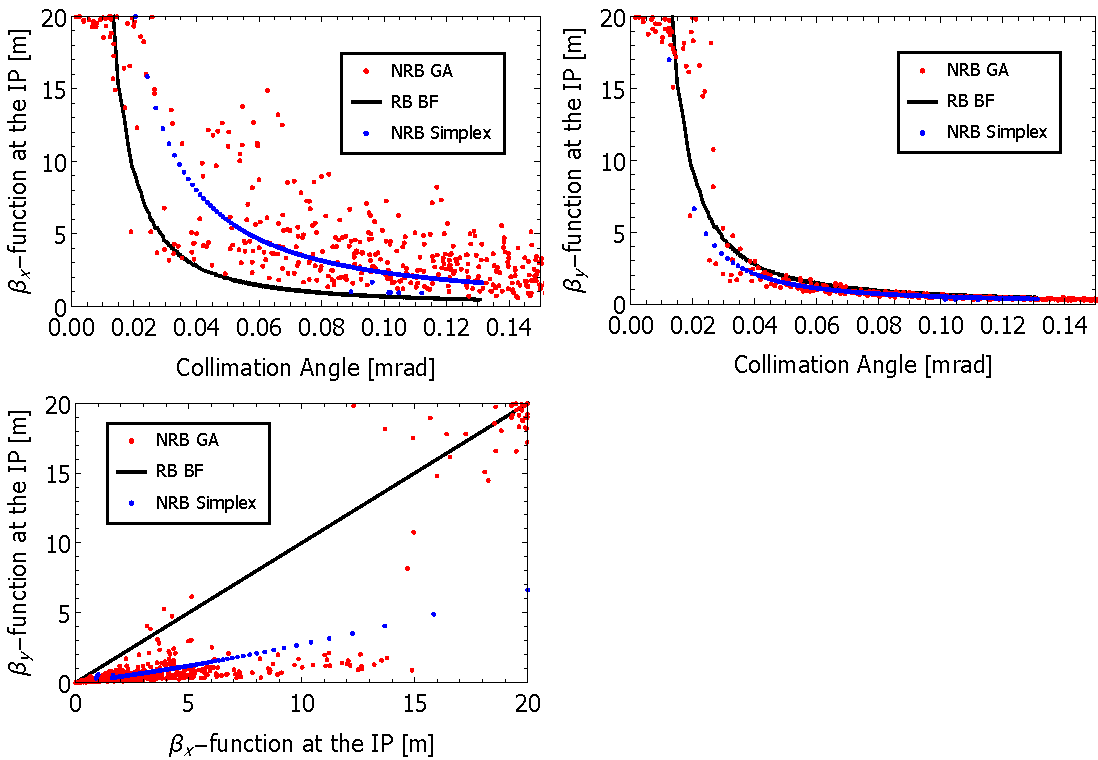
\includegraphics[width=\textwidth]{Figures/DIANA_Inverse_Compton_Source_Design/DIANA717param.pdf}
\caption{DIANA 717~\si{\mega\electronvolt} 2nd turn ICS source optimisations, comparing the two non-round beam approaches (simplex (blue) and GA (red)) and the round beam approach (black). Top Left: parameter space of the interaction $\beta$-function in the $x$ plane and collimation angle for optimised cases. Top Right: parameter space of the interaction $\beta$-function in the $y$ plane and collimation angle for optimised cases. Bottom Left: interaction point $\beta$-function parameter space in the $x$ and $y$ plane for optimised cases. Again, elliptical electron bunches are favoured at the IP, with a larger horizontal beam size because of the laser pulse--electron bunch crossing angle in the horizontal $X$ plane.}
\label{fig:DIANA717_param}
\end{figure}
The 717~\si{\mega\electronvolt} parameter space tuning curves in Fig.~\ref{fig:DIANA717_param} shows similar properties to the parameter space of the 362~\si{\mega\electronvolt} tuning curve in Fig.~\ref{fig:DIANA362_param}. However, the collimation angles decrease in comparison to the 362~\si{\mega\electronvolt} tuning curve because $\theta \propto 1/\gamma$, and hence the decreases with increasing electron beam energy. The bandwidth (Eq.~\ref{eq:RMS_bandwidth}) is dependent on the acceptance angle ($\Psi=\gamma\theta$), therefore the bandwidth does not decrease with increasing electron energy and the concomitant scattering angle reduction. Again, larger horizontal $\beta$-functions are favoured in comparison to the vertical interaction $\beta$-functions ($\beta_{x}>\beta_{y}$) in the non-round optimisations, which means the transverse profile of the electron bunch is elliptical and larger horizontally because of the 5~\si{\degree} crossing angle in the $x$--$z$ plane. Hence, the non-round beam optimisation results are selected because they have not tended to the round beam solution.    

\begin{figure}[!h]
\centering
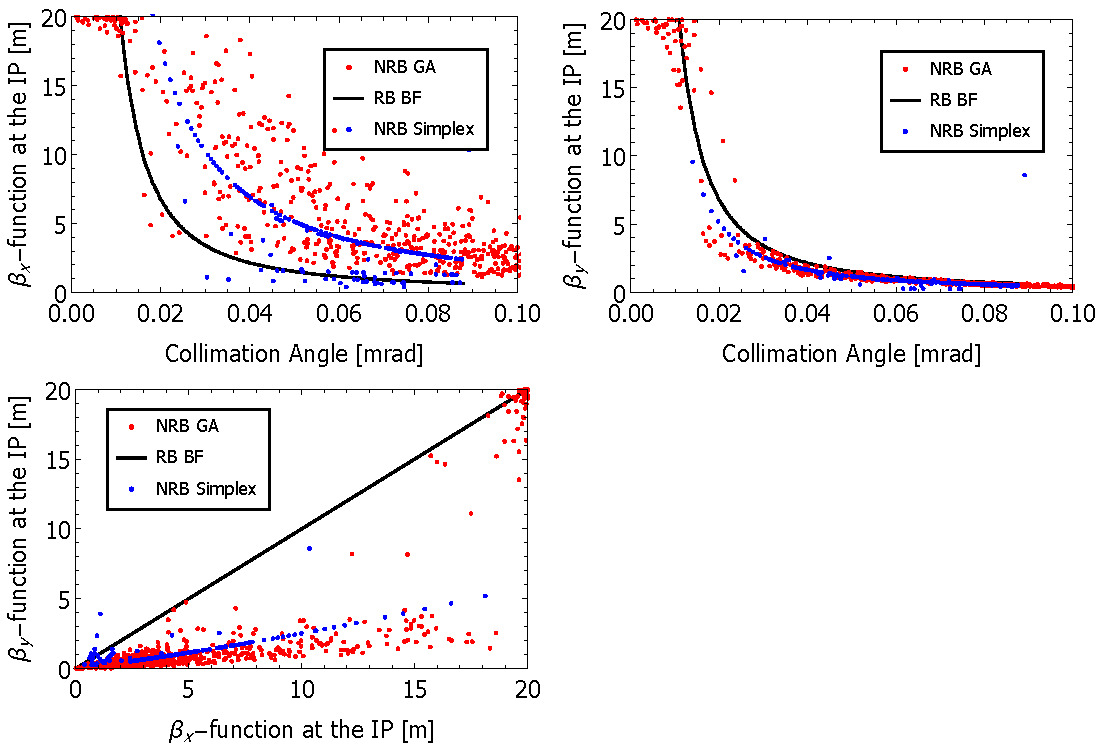
\includegraphics[width=\textwidth]{Figures/DIANA_Inverse_Compton_Source_Design/DIANA1072param.pdf}
\caption{DIANA 1072~\si{\mega\electronvolt} 3rd turn ICS source optimisations, comparing the two non-round beam approaches (simplex (blue) and GA (red)) with the round beam approach (black). Top Left: parameter space of the interaction $\beta$-function in the $x$ plane and collimation angle for optimised cases. Top Right: parameter space of the interaction $\beta$-function in the $y$ plane and collimation angle for optimised cases. Bottom Left: interaction point $\beta$-function parameter space in the $x$ and $y$ plane for optimised cases. Elliptical electron beams with $\beta_{x}^{*} > \beta_{y}^{*}$ are optimal because of the 5~\si{\degree} crossing angle in the $x$--$z$ plane.}
\label{fig:DIANA1072_param}
\end{figure}
Fig.~\ref{fig:DIANA1072_param} shows the parameter space tuning curves corresponding to the optimal collimated flux--\textit{rms} bandwidth tuning curves (in Fig.~\ref{fig:DIANAFBW}) in the range 0--1\% \textit{rms} bandwidth. The Pareto fronts are similarly curved in all $\beta_{x/y}$--$\theta_{\mathrm{col}}$ plots to those at the 362~\si{\mega\electronvolt} and 717~\si{\mega\electronvolt} electron energies however, the collimation angles of the solutions are smaller than the 717~\si{\mega\electronvolt} electron bunch energy case due to the higher electron bunch energy. NRB solutions again produce maximal collimated flux, as shown in the $\beta_{x}$--$\beta_{y}$ plot, with $\beta_{x}>\beta_{y}$ resulting in an elliptical electron bunch spot at the IP. Within the $\beta_x$--$\theta_{\mathrm{col}}$ plot, there are some simplex NRB optimisation points which do not correspond to the overall Pareto front trend, these points appear to be closer to the RB solution and could be points in which the simplex optimisation has failed to converge. 

Overall, for the parameter space tuning curves in Figs.~\ref{fig:DIANA362_param}, \ref{fig:DIANA717_param}, \ref{fig:DIANA1072_param}, the GA NRB and simplex RB solutions show good agreement. The NRB solutions clearly deviate from the RB solutions in each nominal electron bunch energy case with optimal elliptical electron bunch spots at the IP. Hence the NRB optimisation solutions increase the collimated flux of the DIANA ICS source and are the correct optimisation method for the DIANA ICS source. Collimation angle also appears to vary with energy; collimation angles decrease with increasing electron energy because $\theta \propto 1/\gamma$, as explained in Section~\ref{sec:electron_photon_interaction_cross_section}.  

\subsection{Optical Cavity and Laser Pulse Parameters}
\label{sec:DIANA_laser_fabry_perot}

% Why re-circ + Nd:YAG?
A Nd:YAG laser ($\lambda = 1064$~\si{\nano\meter}) is proposed for the DIANA ICS source which is re-circulated using a 4 mirror Fabry-Perot optical cavity with a 5\si{\degree} crossing angle between the electron bunch and laser pulse, as shown in Fig.~\ref{fig:DIANA_interaction}. A re-circulated laser pulse scheme (see Section~\ref{sec:lasers_fabry_perot}), where a c. 100~\si{\micro\joule} laser pulse makes many round trips of an optical cavity is selected to take advantage of the 125~\si{\mega\hertz} repetition rate available from the DIANA ERL electron beam. Explanation of the operation of an ICS source with a Fabry-Perot optical cavity is explained in Section~\ref{sec:lasers_fabry_perot}.

As noted in Section~\ref{sec:lasers_fabry_perot}, the average laser power of the re-circulated scheme is larger than the `single shot' approach, and higher average laser power corresponds to a high-flux ICS source. However, the peak power of the laser pulse in the re-circulate pulse scheme is reduced. Main applications of a $\gamma$-ray ICS source, such as nuclear resonance fluorescence and medical isotope production, require high average power $\gamma$-ray beams not high peak powers therefore the re-circulated scheme is selected. As in the CBETA ICS source design in Chapter~\ref{CBETA_Inverse_Compton_Scattering_Source_Design}, the cERL Fabry-Perot cavity \cite{akagi2016narrow} is used as the model cavity design for the DIANA ICS source and a full optical cavity design is beyond the scope of this thesis.

% 4-mirror + Nd:YAG selection 
Envisioned parameters of the laser pulse provided by a Nd:YAG ($\lambda = 1064$~\si{\nano\meter}) laser and a four mirror Fabry-Perot optical cavity are shown in Table~\ref{tab:DIANA_laser_pulse_design_parameters}. As noted in Section~\ref{sec:lasers_fabry_perot}, a 4 mirror cavity is selected over a 2 mirror design for improved stability of operation and better focal properties. Following the example of the CBETA ICS source in Chapter~\ref{CBETA_Inverse_Compton_Scattering_Source_Design}, an Nd:YAG laser is selected for its relatively short pulse duration ($t_{\mathrm{laser}}=10$~\si{\pico\second}), though longer than femtosecond scale Ti:Sa lasers, narrow spectral bandwidth and because the incident photon energy ($E_{L}=1.17$~\si{\electronvolt}) is sufficient to produce 20~\si{\mega\electronvolt} $\gamma$-rays from \si{\giga\electronvolt}-scale electron bunches. 
\begin{table}[!h]
\centering
\caption{Nd:YAG Gaussian laser pulse parameters at the DIANA ICS IP. The interacted laser pulse is produced via a Nd:YAG infrared laser and re-circulated in a bow-tie Fabry-Perot optical cavity, as shown in Fig.~\ref{fig:DIANA_interaction}.}
\vspace{3mm}
\begin{tabular}{lcc}
\hline\hline
Parameter & Quantity & Unit \\
\hline
Wavelength, $\lambda_\textrm{laser}$ & 1064 & \si{\nano\meter}\\
Photon energy, $E_\textrm{laser}$ & 1.17 & \si{\electronvolt}\\
Pulse energy, $E_{pulse}$  & 100 & \si{\micro\joule}\\
Number of photons, $N_{\textrm{laser}}$ & 5.34$\times 10^{14}$ & \\ 
Repetition rate, $f$ & 125 & \si{\mega\hertz}\\
Spot size at the IP, $\sigma_\textrm{laser}$ & 25 & \si{\micro\meter}\\
Crossing angle, $\phi$ & 5 & deg \\
Pulse length, $\tau_{\mathrm{laser}}$  & 10 & \si{\pico\second}\\
Spectral bandwidth (\textit{rms}), $\Delta E_\textrm{laser}/E_\textrm{laser}$ & $6.57\times 10^{-4}$ &   \\
\hline\hline
\end{tabular}
\label{tab:DIANA_laser_pulse_design_parameters}
\end{table}

% Justification of crossing angle
A crossing angle of 5\si{\degree} is chosen to prevent the scattered $\gamma$-rays and the electron bunches from hitting cavity mirrors. Head-on interactions are possible using chicane interaction regions  that can introduce (remove) the electron bunch to (from) the IP within the mirror spacing (as used in MuCLS \cite{eggl2016munich}) or via mirrors with holes, both described in more detail Section~\ref{sec:fabry_perot_optical_cavities}, but these reduce the stored laser power available to ICS sources and are not selected for the DIANA ICS source. A crossing angle within a 2--12\si{\degree} range is reasonable for integration of cavity mirrors \cite{variola2011luminosity} whilst providing a high flux. A 5\si{\degree} crossing angle is also proposed because it has been demonstrated with the cERL ICS \cite{akagi2016narrow} Fabry-Perot optical cavity used in an ERL, though this angular crossing will reduce the flux of the ICS source (Eq.~\ref{eq:angular_crossing_factor}). 

% Justification of rep freq
The repetition frequency of 125~\si{\mega\hertz} results in a cavity path length of 2.4~\si{\meter} for a single stored laser pulse, which is tolerable for misalignment errors \cite{zomer2009polarization}, and within the same scale as the 9.2~\si{\meter} MuCLS optical re-circulation cavity \cite{eggl2016munich}. The minimum path length limitation of a Fabry-Perot optical cavity is due to mirror heating, which results in thermoelastic deformation of the optical cavity mirrors causing a loss of stability of the optical cavity \cite{chaikovska2016high}. A further discussion of repetition rate is included in Section~\ref{sec:lasers_fabry_perot}.   

% Justification of Spot size
A \textit{rms} spot size (radius) on the order of 10's~\si{\micro\meter} is common in ICS sources \cite{deitrick2017inverse,drebot2019brixs,dupraz2020thomx}; for example the laser pulse spot size achieved at cERL ICS is 20~\si{\micro\meter}/30~\si{\micro\meter} \cite{akagi2016narrow}, which is similar to the parameters proposed here for the DIANA ICS source. The waist size of the DIANA ICS source is within the state-of-the-art and smaller waists are difficult to achieve because of astigmatism in mirrors \cite{zomer2009polarization}, and because the laser pulse spot size at the cavity mirrors increases as the laser spot size decreases due to the Rayleigh range (Eq.~\ref{eq:rayleigh_range}) by $\sigma_{w} = \sigma_{L}\sqrt{1+\frac{z_{L}}{z_{R}}}$.

% Justification of cavity + stored power
These laser pulse parameters are based upon the demonstration of the Fabry-Perot optical cavity in the cERL ICS experiment \cite{akagi2016narrow}, however they have been modified for a reduced 125~\si{\mega\hertz} repetition rate with an increased pulse energy of 100~\si{\micro\joule}, resulting in an average stored power of 12.5~\si{\kilo\watt} re-circulated in the optical cavity. Therefore, the stored power of the Fabry-Perot cavity in the DIANA ICS source is increased relative to the 10~\si{\kilo\watt} CBETA ICS source design in Table~\ref{tab:CBETA_laser_pulse_design_parameters}, which increases the flux of scattered photons produced from the DIANA ICS source. The increased laser pulse power is within the MuCLS demonstration of 70~\si{\kilo\watt} \cite{eggl2016munich} and the DIANA optical re-circulation cavity also has an average stored laser power a factor of $\sim50\times$ lower than the 670~\si{\kilo\watt} average stored power demonstrated by Carstens et al \cite{carstens2014megawatt} at 250~\si{\mega\hertz}. Therefore, the laser pulse energy and repetition rate (average stored laser power) appear to be feasible and are based on previously demonstrated parameters for ICS sources. 

% Justification of the spectral bandwidth
The \textit{rms} wavelength spread of the proposed incident laser pulse (based on commercial Nd:YAG lasers \cite{thorlabs2021ndyag200}) is small ($\Delta\lambda = 0.7$~\si{\nano\meter}) \cite{corner2019} resulting in a small spectral bandwidth of $\Delta E_{L}/E_{L} = 6.57\times 10^{-4}$. Small spectral bandwidth is necessary to give a narrowband ICS source as the bandwidth of the scattered radiation (Eq.~\ref{eq:RMS_bandwidth}) is dependent upon the spectral bandwidth. Comparatively, other lasers have a larger spectral bandwidth (see Section~\ref{sec:lasers_fabry_perot}) therefore the Nd:YAG laser is practical for development of a narrowband ICS source. 

\section{ICS Source Spectral Output}
\label{sec:DIANA_spectral_output}

The anticipated spectral output of the DIANA ICS source is shown in Table~\ref{tab:DIANA_spectral_output} using the electron bunch and laser pulse parameters specified in Tables~\ref{tab:DIANA_electron_beam_design_parameters},~\ref{tab:DIANA_laser_pulse_design_parameters}. The spectral output parameters are shown for both the 0.5\% \textit{rms} bandwidth optimised configuration, using the simplex NRB method of Section~\ref{sec:NRB_optimisation}, and the baseline configuration that has small electron bunch spot sizes and constant $\beta$-functions ($\beta_{x/y}=0.2$~\si{\meter}). The average and peak brilliance, spectral density and uncollimated flux have been calculated for the baseline case. The collimated flux can only be calculated for the 0.5\% \textit{rms} bandwidth configuration because the baseline case is used to define the full, uncollimated radiation spectrum. All calculation methods are outlined in Chapter~\ref{Photon_Production_by_Inverse_Compton_Scattering}. 
\begin{table}[!h]
\caption{Anticipated photon output for each of the three nominal electron beam energies (at each turn) in DIANA, assuming a 5\si{\degree} crossing angle. The recoil parameter is small ($X < 0.02$) even at 1072~\si{\mega\electronvolt}. The collimated flux has been optimised for a 0.5\% \textit{rms} bandwidth using the NRB simplex optimisation (see Section~\ref{sec:NRB_optimisation}) and the baseline case achieves  $\beta^{*} =0.2$~\si{\meter} at the IP to for each electron energy.}
\vspace{3mm}
\centering
\begin{threeparttable}
\begin{tabular}{lcccc}
\hline\hline
 & \multicolumn{3}{c}{Electron Kinetic Energy (\si{\mega\electronvolt})} & \\
 \cline{2-4}
 & 362 & 717 & 1072 & \\
\hline
$\gamma$-ray peak energy  & 2.33 & 9.06 & 20.11 & \si{\mega\electronvolt}\\
\hline
 & \multicolumn{3}{c}{Baseline} & \\
\hline
Source size ($x$/$y$)  & 10.72/10.72 & 8.00/8.00 & 6.65/6.65 & \si{\micro\meter} \\
Uncollimated flux  & 5.77$\times 10^{10}$ & 6.02$\times 10^{10}$ & 6.08$\times 10^{10}$ & ph/\si{\second}\\
Spectral density  & 2.48$\times 10^{5}$ & 6.65$\times 10^{4}$ & 3.03$\times 10^{4}$ & ph/\si{\second} \si{\electronvolt}\\
Average brilliance  & 5.64$\times 10^{12}$ & 2.05$\times 10^{13}$ & 4.45$\times 10^{13}$ & ph/\si{\second} \si{\milli\meter}$^{2}$\si{\milli\radian}$^{2}$ 0.1\% bw\\
Peak brilliance\tnote{*}  & 4.44$\times 10^{18}$ & 1.62$\times 10^{19}$ & 3.50$\times 10^{19}$ & ph/\si{\second} \si{\milli\meter}$^{2}$ \si{\milli\radian}$^{2}$ 0.1\% bw\\
\hline
 & \multicolumn{3}{c}{0.5\% \textit{rms} bandwidth} & \\
\hline
Source Size ($x$/$y$) & 19.36/12.54 & 19.35/12.52 & 19.33/12.50 & \si{\micro\meter} \\ 
Collimated flux  & 1.30$\times 10^{9}$ & 1.29$\times 10^{9}$ & 1.29$\times 10^{9}$ & ph/\si{\second} 0.5\% bw \\
\hline\hline
\end{tabular}
\begin{tablenotes}
\item[*]{(Eq.~\ref{eq:peak_brilliance}) is used to calculate the peak brilliance.}
\end{tablenotes}
\end{threeparttable}
\label{tab:DIANA_spectral_output}
\end{table}

% what energies are possible + tunability
Table~\ref{tab:DIANA_spectral_output} shows that the DIANA ICS source is capable of producing $\gamma$-rays up to 20.11~\si{\mega\electronvolt} ($E_{e}=1072$~\si{\mega\electronvolt}), with the first two turns ($E_{e} = $362, 717~\si{\mega\electronvolt}) producing 2.33 and 9.06~\si{\mega\electronvolt} $\gamma$-rays respectively. The crossing angle ($\phi=5\si{\degree}$) of the ICS interaction in DIANA reduces the maximum scattered photon energy from 20.14~\si{\mega\electronvolt} to 20.11~\si{\mega\electronvolt} -- a small $\sim 30$~\si{\kilo\electronvolt} reduction. Depending on the tunability of the electron bunch and through variation of the scattering angle sampled (due to the energy--angle correspondence), scattered photon energies from 1--20.11~\si{\mega\electronvolt} may be accessible, i.e  a steplessly variable tunablility. 

% Why is flux, spec den, avg brill good 
World-leading uncollimated flux, spectral density and average brilliance are available from the DIANA ICS source due to the interaction of a high brightness (small emittance, high bunch charge) electron beam with a re-circulated laser pulse at high repetition rate. For example, the maximum flux of HI$\gamma$S \cite{weller2009research}, the current highest flux $\gamma$-ray ICS source, is $\mathcal{F} =5\times 10^{8}$~ph/\si{\second}, a factor of $\sim 120$ smaller than the maximum flux of the DIANA ICS source. A full comparison of the DIANA ICS source to other designed and operated ICS sources on the \si{\mega\electronvolt}-scale in terms of scattered photon energies and flux is presented in Section~\ref{sec:gamma_ICS_comparison}. 

Flux reduces by 5.1\% from the 1072~\si{\mega\electronvolt} to the 362~\si{\mega\electronvolt} electron energy because of the increase in the electron bunch spot size at lower energies. The increase in the recoil parameter (Eq.~\ref{eq:X_geometry}) decreases the flux negligibly. The variation with energy of average and peak brilliance is
due to the Lorentz transformation  causing a $\mathcal{B}\propto \gamma^{2}$ (shown in (Eq.~\ref{eq:average_brilliance_compact})). Spectral density (Eq.~\ref{eq:spectral_density}) deceases with increasing electron beam energy as the spectral density is the flux per unit scattered photon energy and the scattered photon energy (Eq.~\ref{eq:scattered_photon_energy}) is double Doppler shifted, yielding a $\mathcal{S}\propto 1/\gamma^{2}$ dependence.  

Calculation of the flux, spectral density and (average and peak) brilliance of the DIANA ICS source all take into account the geometric luminosity reduction which arises because of the reduction in laser pulse--electron bunch overlap from an angular crossing and the hourglass effect, where the spot size of the diverging electron bunch and laser pulse varies throughout the interaction. Both effects are further explained in Section~\ref{sec:geometric_luminosity_reduction}. The 5~\si{\degree} crossing angle imposed on the interaction and the divergence of the electron bunch and laser pulse cause a factor of $\sim10$ reduction ($R_{ACHG}=0.094$ \cite{miyahara2008luminosity}) in the luminosity of the interaction. The hourglass effect is suppressed in the DIANA ICS source because the angular crossing results in a small overlap between the electron bunch and laser pulse and within the overlap the electron bunch and laser pulse diverge negligibly.  

% Why is peak brilliance poor?
Peak brilliance of the DIANA ICS source is reduced in the DIANA ICS source in comparison to other proposed ICS sources \cite{barty2011overview} with $\mathcal{B}_{\mathrm{pk}}>10^{20}$~ph/\si{\second}~\si{\milli\meter}$^{2}$--\si{\milli\radian}$^{2}$~0.1\% BW because DIANA favours average brilliance over peak brilliance, which is more useful for the applications listed in Section~\ref{sec:DIANA_ICS_applications}. The modest peak brilliance of DIANA is due to the low energy of the interacted laser pulse ($E_{\mathrm{pulse}} = 100$~\si{\micro\joule}) and the moderate picosecond durations of the laser pulse ($\tau_{L}=10$~\si{\pico\second}) and electron bunch ($\tau_{e}=3$~\si{\pico\second}). High peak brilliance ICS sources, such as the original ELI-NP-GBS design \cite{adriani2014technical}, typically target femtosecond electron bunch and laser pulse lengths with Joule-scale laser pulse energies with the `single shot' ICS source approach. However, a high repetition rate enables DIANA to produce a high average brilliance of up to $\mathcal{B}_{\mathrm{avg}}=4.45\times 10^{13}$~ph/\si{\second}~\si{\milli\meter}$^{2}$--\si{\milli\radian}$^{2}$~0.1\% BW. 

% Single point Narrowband optimisation 
The three nominal electron energy ($E_{e}=$ 362, 717, 1072~\si{\mega\electronvolt} ) DIANA ICS sources have been optimised for a 0.5\% \textit{rms} bandwidth using the non-round beam simplex optimisation method, described in Chapter~\ref{Optimisation_and_Characterisation_of_Inverse_Compton Scattering_Spectra}, because this optimisation method delivers a higher collimated flux (albeit a small $<1$\% variation from the GA method). The optimised electron beam interaction $\beta$-functions and collimation angles resulting from the 0.5\% \textit{rms} bandwidth optimisation are shown in Table~\ref{tab:DIANA_electron_beam_design_parameters}, the collimated flux is calculated using these parameters.

The DIANA ICS source is expected to deliver a collimated flux of 1.30$\times 10^{9}$~ph/\si{\second} in a 0.5\% \textit{rms} bandwidth. As the $\beta$-functions are allowed to vary with electron energy in the optimisations, the increase in flux due to the decreasing electron spot size with electron energy observed in the baseline case in Table~\ref{tab:DIANA_spectral_output} is not observed for the optimised case. The RB optimisation (see Section~\ref{sec:RB_optimisation}) for the 1072~\si{\mega\electronvolt} electron bunch energy predicts a collimated flux of $1.24\times 10^{9}$~ph/\si{\second} in comparison to the $1.30\times 10^{9}$~ph/\si{\second} for the NRB simplex optimisation, therefore a small gain in flux of $\sim5$\% is achieved via NRB simplex optimisation; similar differences are achieved for the other nominal electron energies. Collimation also has another benefit as at a collimator, placed 10~\si{\meter} downstream of the interaction point, the spot size (radius) of the radiation produced in a 0.5\% \textit{rms} bandwidth with the 1072~\si{\mega\electronvolt} electron bunch is 0.61~\si{\milli\meter}, therefore DIANA could produce a small spot (pencil beam) of $\gamma$-rays for experimental use. A small $\gamma$-ray spot is useful experimentally for imaging small samples or for example detecting small features in nuclear waste canisters with nuclear resonance fluorescence \cite{angell2015demonstration}.  

To further characterise narrowband operation of the DIANA ICS sources a series of optimised tuning curves are produced at each nominal electron energy, based on optimisation methods in Chapter~\ref{Optimisation_and_Characterisation_of_Inverse_Compton Scattering_Spectra}, to show the maximum collimated flux as a function of bandwidth within the narrow bandwidth ($<1$\% \tetxit{rms} BW) regime. For these optimisations, the laser pulse parameters remain unchanged from Table~\ref{tab:DIANA_laser_pulse_design_parameters} and only the $\beta$-functions at the IP in each plane and the collimation angle are varied. The solution space tuning curves (Pareto-optimal fronts) of the collimated flux--\textit{rms} bandwidth in the narrowband range ($\Delta E_{\gamma}/E_{\gamma} < 1$\%) are shown in Fig.~\ref{fig:DIANA_FBW}, with the corresponding parameter space fronts previously presented in Figs.~\ref{fig:DIANA362_param}, \ref{fig:DIANA717_param}, \ref{fig:DIANA1072_param} and discussed in Section~\ref{sec:sec:DIANA_electron_parameters}.  
\begin{figure}[!h]
\centering
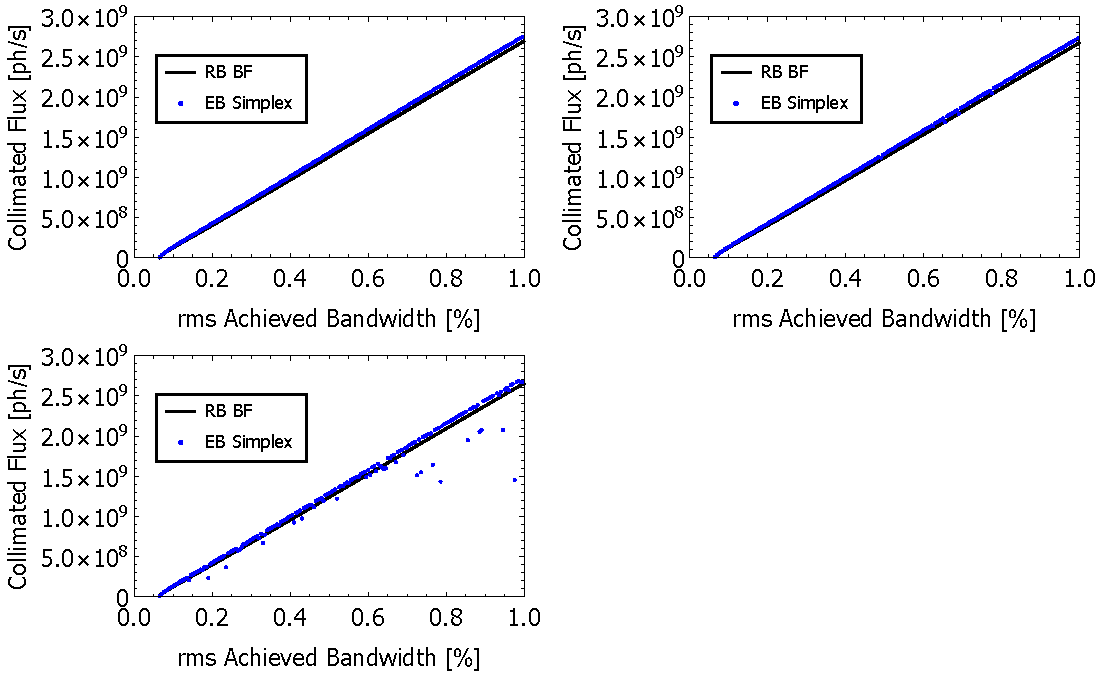
\includegraphics[width=\textwidth]{Figures/DIANA_Inverse_Compton_Source_Design/DIANAFBW.pdf}
\caption{Collimated flux--\textit{rms} bandwidth tuning curves (Pareto-optimal fronts) for the three optimisations methods: round beam (RB BF, black), non-round beam genetic algorithm (NRB GA, red) and non-round beam simplex (NRB Simplex, blue) in Sections~\ref{sec:RB_optimisation}, \ref{sec:NRB_optimisation} for the three nominal electron bunch energies ($E_{e}=362,~717,~1072$~\si{\mega\electronvolt}) of the DIANA ICS source. Top Left: 362~\si{\mega\electronvolt} electron bunch. Top Right: 717~\si{\mega\electronvolt} electron bunch. Bottom Left: 1072~\si{\mega\electronvolt} electron bunch.}
\label{fig:DIANA_FBW}
\end{figure}

Fig~\ref{fig:DIANA_FBW} shows that the Pareto fronts of the collimated flux--\textit{rms} bandwidths are in good agreement with the simplex and genetic algorithm methods for each of the three nominal electron energies ($E_{e}= $362, 717, 1072~\si{\mega\electronvolt}). A small increase in collimated flux is observed for the NRB optimisations in comparison to the RB optimisations; however, the increase is small ($\sim5$\%) as a round beam approximation is a good approximation for an ERL due to the small emittance and $\beta$-functions at the IP. The increase in flux for NRB optimisation in comparison to RB optimisation increases as a function of \textit{rms} bandwidth -- at a 1\% bandwidth the collimated flux from a NRB optimisation is increased by 7\% whereas at 0.2\% bandwidth the increase is around 2\%.  

The solution space tuning curves (collimated flux vs \textit{rms} bandwidth) for each electron energy are near-identical and small variation in the tuning curves is observed because of differing recoil parameters, which reduce the collimated flux by reducing the cross section. For example the recoil parameter (Eq.~\ref{eq:X_geometry}) of the 362~\si{\mega\electronvolt} electron beam (head-on, backscattering) is $X_{362~\si{\mega\electronvolt}}=6.51\times 10^{-3}$ whereas for the 1072~\si{\mega\electronvolt} the recoil parameter is $X_{1072~\si{\mega\electronvolt}}=0.0193$. As explained for the single point 0.5\% \textit{rms} bandwidth optimisations in Table~\ref{tab:DIANA_spectral_output}, spot size reduction with energy -- a factor in flux variation with energy in the baseline case -- is not relevant here as the $\beta$-functions at the IP are allowed to vary.

A collimated flux of up to $\mathcal{F}_{\mathrm{col}}\approx$2.7$\times 10^{9}$~ph/\si{\second} can be produced by DIANA in a narrow bandwidth ($<1$\%), practically independently of electron bunch energy. The minimum achievable bandwidth (the cut-off bandwidth in Fig.~\ref{fig:DIANA_FBW}) in each of the three nominal electron energy tuning curves is identical; the low bandwidth limit (Eq.~\ref{eq:bandwidth_limitation_minimum}) is imposed by the energy spread of the electron bunch ($\Delta E_{e}/E_{e} = 5\times 10^{-5}$) and the spectral bandwidth of the laser pulse ($\Delta E_{L}/E_{L}=6.57\times 10^{-4}$) and is given by   
\begin{equation*}
\left(\frac{\Delta E_{\gamma}}{E_{\gamma}}\right)_{\mathrm{min}} \approx \sqrt{\left[\left(\frac{2+X}{1+X}\right)\frac{\Delta E_{e}}{E_{e}}\right]^{2} + \left[\left(\frac{1}{1+X}\right)\frac{\Delta E_{L}}{E_{L}}\right]^{2}}.
\end{equation*}
For example, the minimum bandwidth of the 1072~\si{\mega\electronvolt} nominal electron energy ICS source is $\left(\Delta E_{\gamma}/E_{\gamma}\right)_{\mathrm{min}} \approx 10^{-3}$ which is approximately the low bandwidth cut-off in all of the plots in Fig.~\ref{fig:DIANA_FBW}. 
   
The three nominal electron energy ICS sources driven by the proposed DIANA 3-turn ERL have been characterised by spectrum plots within a 0.5\% \textit{rms} bandwidth for a single electron bunch--laser pulse interaction, using the \textsc{ICARUS} code as described in Chapter~\ref{Optimisation_and_Characterisation_of_Inverse_Compton Scattering_Spectra}. \textsc{ICARUS} has previously been benchmarked against the semi-analytical ICS spectrum code \textsc{ICCS3D} \cite{krafft2016laser,ranjan2018simulation} for both the CBETA ICS in Section~\ref{sec:CBETA_spectral_output} and a series of test cases in Section~\ref{sec:benchmarking_cases_characterisation_optimisation}. The optimised parameters for the simplex NRB optimisation, as shown in Table~\ref{tab:DIANA_electron_beam_design_parameters}, are used to produce the spectra of the DIANA ICS source. A head-on ($\phi=0$) interaction is modelled, therefore the Compton edge scattered photon energies (Eq.~\ref{eq:compton_edge_energy}) -- the scattered photon energy at peak spectral density -- are higher than the $\gamma$-ray peak energies shown in Table~\ref{tab:DIANA_spectral_output}. For example the scattered photon energy is increased by 30~\si{\kilo\electronvolt} for the DIANA 1072~\si{\mega\electronvolt} electron bunch. Since a head-on interaction is modelled, the reduction in spectral density (flux) by the angular crossing (Eq.~\ref{eq:angular_crossing_factor}) is also neglected, which has a value of $R_{AC}=0.143$ for the optimised 1072~\si{\mega\electronvolt} electron beam.
The electron bunch and laser pulse are also modelled as Gaussian distributions, with emittance and energy spread (laser pulse and electron bunch) effects accounted for. Spectra for the DIANA ICS sources at 0.5\% \textit{rms} bandwidth are shown in Fig~\ref{fig:DIANA_spectra}.
\begin{figure}[!h]
\centering
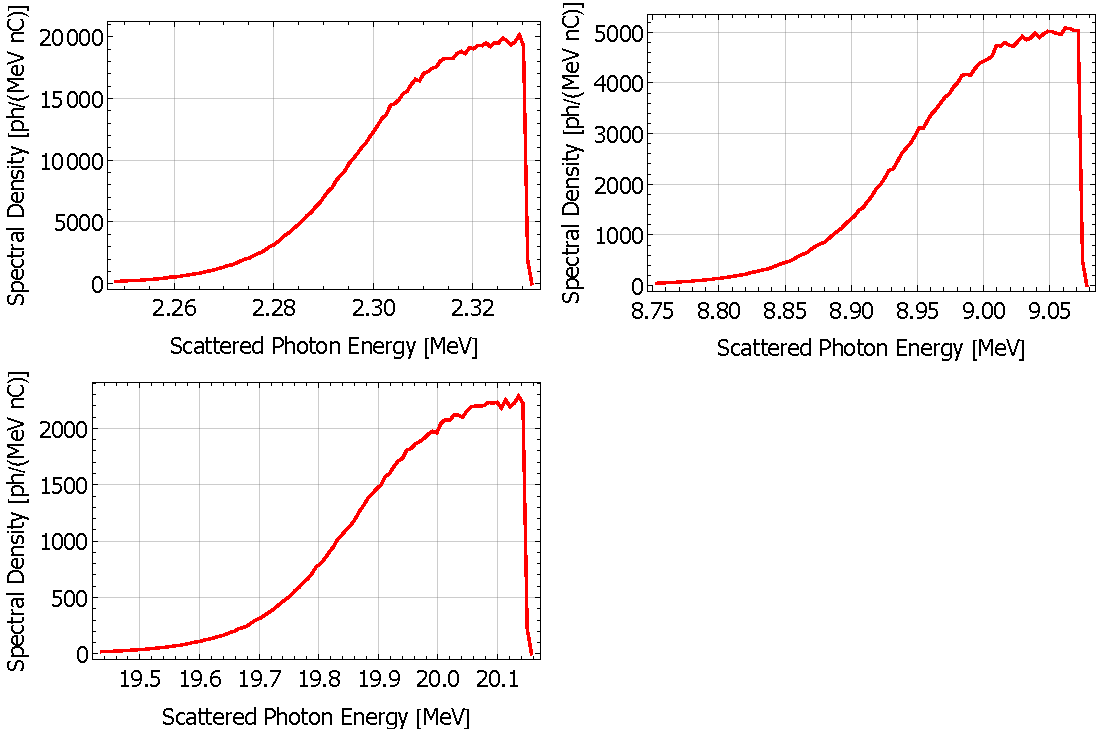
\includegraphics[width=\textwidth]{Figures/DIANA_Inverse_Compton_Source_Design/DIANA_spectra.pdf}
\caption{Predicted spectral output (flux) of 1064~\si{\nano\meter} incident photons interacting head-on ($\phi=0$) with each of the three nominal energy electron bunches in DIANA; this spectrum was generated using the \textsc{ICARUS} code. Top Left: 362~\si{\mega\electronvolt}  electron bunch--laser pulse interaction spectrum, with peak energy $E_{\gamma}=2.33$~\si{\megaelectronvolt} and an angular crossing luminosity reduction factor (Eq.~\ref{eq:angular_crossing_factor}) $R_{AC}=0.143$. Top Right: 717~\si{\mega\electronvolt}  electron bunch--laser pulse interaction spectrum, with peak energy $E_{\gamma}=9.07$~\si{\mega\electronvolt} and an angular crossing luminosity reduction factor  $R_{AC}=0.143$. Bottom Left: 1072~\si{\mega\electronvolt}  electron bunch--laser pulse interaction spectrum, with peak energy $E_{\gamma}=20.13$~\si{\mega\electronvolt} and an angular crossing luminosity reduction factor $R_{AC}=0.142$. The scattered photon energy of the maximum spectral density corresponds to the Compton edge energy (Eq.~\ref{eq:compton_edge_energy}), where the incident photons are backscattered ($\theta = 0$). }
\label{fig:DIANA_spectra}
\end{figure}

The spectra of the DIANA ICS source at each of the three nominal energies ($E_{e} = $362, 717, 1072~\si{\mega\electronvolt}) are similar in shape; they differ significantly in both spectral density and scattered photon energy. The Compton edge (Eq.~\ref{eq:compton_edge_energy}) is defined as the energy of the scattered photons originating from backscattered incident photons and this coincides with the peak spectral density of the spectra. The scattered photon energies (Eq.~\ref{eq:scattered_photon_energy}) vary due to $E_{\gamma}\propto\gamma^{2}$ and the scattered photon energies at the Compton edge (Eq.~\ref{eq:compton_edge_energy}) of the spectrum agree with the calculated values in Table~\ref{tab:DIANA_spectral_output}. Scattered photon energies above the Compton edge (Eq.~\ref{eq:compton_edge_energy}) are produced because electrons and incident laser photons exist with energies above the mean electron bunch energy -- a high scattered photon energy tail. A section of the total ICS interaction spectrum is selected by the collimator (in this case the 0.5\% \textit{rms} bandwidth section), therefore the scattered photon energies with scattering angles beyond the collimation angle are removed. For example, for the 1072~\si{\mega\electronvolt} electron bunch scattered photons with scattering angles larger than the  $\theta_{\mathrm{col}} = 0.061~\si{\milli\radian}$ collimation angle are collimated, corresponding to $E_{\gamma} = 19.8$~\si{\mega\electronvolt}.However, a low scattered photon energy tail consisting of scattered photons $E_{\gamma} < 19.8$ is observed. The low scattered photon energy tail occurs due to interactions with 
electrons with lower energies than the mean and because the scattered photons are not emitted from a point source -- the electron bunch has a finite emittance which allows photons to pass through the collimator with scattering angles larger than the collimation angle.

The peak spectral density of the DIANA ICS sources in the spectrum is decreased at larger electron bunch energies as the spectral density (Eq.~\ref{eq:spectral_density}) $\mathcal{S} \propto 1/\gamma^{2}$ -- the spectral density is the flux per unit scattered photon energy and there is a $\gamma^{2}$ dependence in the scattered photon energy (Eq.~\ref{eq:scattered_photon_energy}). The spectra in Fig.~\ref{fig:DIANA_spectra} are not smooth because of oscillatory integration errors within the \textsc{ICARUS} code (see Section~\ref{sec:benchmarking_cases_characterisation_optimisation}).

The collimated flux resulting from yield calculations of the \textsc{ICARUS} spectra at each nominal electron energy (for 0.5\% \textit{rms} bandwidth), including $R_{AC} \approx 0.14$, are
\begin{align}
\mathcal{F}_{\mathrm{col}}^{362~\si{\mega\electronvolt}} &= 1.31\times 10^{9}~\mathrm{ph}/\si{\second} \\
\mathcal{F}_{\mathrm{col}}^{717~\si{\mega\electronvolt}} &= 1.30\times 10^{9}~\mathrm{ph}/\si{\second} \\
\mathcal{F}_{\mathrm{col}}^{1072~\si{\mega\electronvolt}} &= 1.29\times 10^{9}~\mathrm{ph}/\si{\second}
\end{align}
which are in close agreement with the collimated fluxes calculated analytically (Eq.~\ref{eq:collimated_flux}) in Table~\ref{tab:DIANA_spectral_output}. Small variations are expected between the analytical collimated flux and the collimated flux calculated from \textsc{ICARUS} spectra as the analytical calculation does not account for energy spread of the electron bunch or laser pulse spectral bandwidth. As the energy spread of the electron bunch and spectral bandwidth of the laser pulse are very small we see good agreement.

\section{Gamma-ray ICS Source Comparison}
\label{sec:gamma_ICS_comparison}

Inverse Compton scattering sources for production of $\gamma$-rays have been designed and demonstrated worldwide and comparison of these against the DIANA ICS source is indicative of the benefits of the ERL driven ICS approach. Differing approaches for ICS production of $\gamma$-rays have been trialed with varying types of accelerators and incident photon sources. For example, the HI$\gamma$S source uses radiation produced from a free electron laser as the incident photon source to achieve high energy photon production up to 100~\si{\mega\electronvolt} \cite{weller2009research}. ICS sources may also have different design goals; for example, ICS sources may be designed for high peak brilliance, which requires high flux per shot and short pulse duration (e.g. 10's \si{\femto\second}), for destructive inspection of samples. Some sources may favour the high peak brilliance approach of a `single shot' design whereas some favour the `re-circulated pulse' approach leading to high average brilliance used for time-averaged measurements e.g. nuclear resonance fluorescence studies. The two main conventional laser ICS source approaches are detailed in Section~\ref{sec:lasers_fabry_perot}. The most relevant $\gamma$-ray ICS facilities for comparison to the DIANA ICS source are those producing $\gamma$-ray radiation with scattered photon energies on the \si{\mega\electronvolt}-scale ($E_{\gamma}>1$~\si{\mega\electronvolt}); a selection of these sources are given in Table~\ref{tab:gammaray_ICS_comparison}. 
\begin{table}[!h]
\caption{Comparison of existing and proposed $\gamma$-ray ICS sources.}
\begin{threeparttable}
\resizebox{\columnwidth}{!}{
\begin{tabular}{lccc}
\hline\hline
ICS & Accelerator Type & Scattered Photon Energy (\si{\mega\electronvolt}) & Flux (ph/\si{\second}) \\
\hline
DIANA\tnote{*} & ERL & 2.33--20.11 & 5.77--6.08$\times 10^{10}$ \\ 
NIJI-IV \cite{sei2017demonstration} & Storage Ring & 1.2 & 3.1$\times 10^{4}$ \\
VIGAS\tnote{*} \cite{shi2021vigas,brenner2020summary} & Linac & 0.2--4.8 & 1--4$\times 10^{8}$ \\
ELI-NP-GBS\tnote{*} \cite{adriani2014technical} & Linac & 0.2--19.5 & $3.9\times 10^{9}$ \\
ELI-NP VEGA\tnote{*} \cite{tanaka2020current,elinp2019vega} & Storage Ring & 1--19.5 & 1$\times 10^{11}$\\
NewSUBARU \cite{utsunomiya2015gamma} & Storage Ring & 5--40 & $3\times 10^{7}$ \\
%VELOCIRAPTOR & Linac & & \\
%T-REX & Linac & & \\
Pan et al CBS\tnote{*} \cite{pan2019design} & Storage Ring & 4--10 & 0.14--3.87$\times 10^{12}$ \\ 
Super-ACO \cite{nutarelli1998gamma} & Storage Ring & 33.4 & $5\times10^{6}$ \\
HI$\gamma$S \cite{weller2009research} & Storage Ring & 1--100 & 5$\times 10^{7}$--5$\times 10^{8}$ \\
\hline\hline
\end{tabular}}
\begin{tablenotes}
\item[*]{Design parameters for sources which are not yet demonstrated.}
\end{tablenotes}
\end{threeparttable}
\label{tab:gammaray_ICS_comparison}
\end{table}

% How does DIANA measure up? ENERGY
The DIANA ICS source is designed to produce $\gamma$-rays across a wide range of scattered photon energies ($E_{\gamma}=$ 2.33--20.11~\si{\mega\electronvolt}), and will be designed to be steplessly variable -- any scattered photon energy in this range will be accessible within this range -- via adjustment of the electron bunch energy. The tunability proposed for the DIANA ICS matches the tunability of the ELI-NP-VEGA system \cite{tanaka2020current,elinp2019vega}, with a similar scattered photon energy range. Other ICS sources such as NewSUBARU and HI$\gamma$S are capable of producing $\gamma$-rays up to 40~\si{\mega\electronvolt} and 100~\si{\mega\electronvolt} respectively, extending the utility of those sources into the nuclear photonics regime \cite{budker2021expanding}. High-energy photon capabilities are possible at NewSUBARU and HI$\gamma$S because of two approaches: the use of frequency doubled lasers at short wavelengths (for example a 2nd harmonic Nd:YAG laser ay $\lambda = 532$~\si{\nano\meter}) or using short-wavelength radiation from an FEL. The former approach is implementable within the current design of the DIANA ICS sources and is a suitable topic for further study, but use of frequency doubled lasers in Fabry-Perot optical cavities poses additional challenges for high average stored power (see Section~\ref{sec:lasers_fabry_perot}).

% Re-circulation advantage and the abundance of storage ring driven ICS
$\gamma$-ray ICS sources designed and/or demonstrated have yet utilised the ERL approach, and in-depth consideration of an ERL as the driver of an inverse Compton scattering source for production of $\gamma$-rays is limited. Predominantly, ICS $\gamma$-ray production is driven by storage rings, with existing ICS sources, such as NewSUBARU \cite{utsunomiya2015gamma} and HI$\gamma$S \cite{weller2009research} utilising existing synchrotron facilities. The European flagship ELI-NP $\gamma$-ray source plans to utilise the Lyncean Technologies variable energy gamma-ray (VEGA) system \cite{tanaka2020current,elinp2019vega} -- a storage ring system instea of the previous ELI-NP-GBS \cite{adriani2014technical} linac system, so next generation ICS sources are still using the storage ring approach. Storage ring sources are undoubtedly favoured because of the high flux available due to re-circulation of the electron bunch and laser pulse leading to a much higher interaction rate. However, as demonstrated in the DIANA ICS source design re-circulation from ERL driven ICS sources can match the high flux operation of storage ring driven ICS sources. The predicted flux of the DIANA ICS source is similar to leading storage ring designs such as ELI-NP VEGA and the CBS \cite{pan2019design} in Table~\ref{tab:gammaray_ICS_comparison}. Therefore, the ERL driven ICS source approach deserves further scrutiny, as multi-turn ERLs such as the proposed PERLE \cite{angal2018perle} and CEBAF \cite{meot2016er} ERLs can offer the necessary higher electron energies ($E_{e} > 250$~\si{\mega\electronvolt}) and ERLs in general may offer more brilliant electron beams \cite{adolphsen2022european} for development of a high flux, narrowband $\gamma$-ray source. 

% How does DIANA measure up? FLUX
DIANA is competitive with other world-leading source designs, such as those by Pan et al \cite{pan2019design} and the ELI-NP-VEGA collaboration \cite{elinp2019vega,tanaka2020current}. The DIANA ICS source flux of 6.08$\times 10^{10}$ph/\si{\second} is bested by both the Compton Back-scattering Source (CBS) by Pan et al \cite{pan2019design}, where a factor of 2 larger laser pulse energy is stored, and the ELI-NP-VEGA source, which is also expected to use a high average stored power cavity beyond the average stored power of DIANA. Head-on ($\phi=0$) interactions are also assumed in the highest flux sources (ELI-NP-VEGA and CBS); the implementation of these are not adequately explained as it is unclear whether the Fabry-Perot optical cavities in each design will have the electron bunches enter within the cavity (via a dipole bend contained in the cavity) or by using holes in the optical cavity mirrors. Both pose issues for optical cavity development as explained in Section~\ref{sec:lasers_fabry_perot}. In the Pan et al CBS design\cite{pan2019design} the hourglass effect (Eq.~\ref{eq:furman_hourglass_reduction}) has been neglected, and this would be non-negligible because the electron bunch and laser pulse are both of considerable length ($\sigma_{z,e} = 110$~\si{\milli\meter}, $\sigma_{z,L} = 6$~\si{\milli\meter}) resulting in an hourglass effect luminosity reduction factor (Eq.~\ref{eq:furman_hourglass_reduction}) of $R_{HG} = 0.66$ (a 34\% reduction in luminosity). In summary, the DIANA ICS source is capable of similar flux performance as the ELI-NP-VEGA and CBS sources, with an angular crossing IP arrangement and demonstrated laser parameters. 

% ERL advantages in bandwidth
Whilst the ERL approach has been shown to be competitive in terms of flux, an ERL driven ICS source may also be more advantageous in achieving a narrow bandwidth and a large collimated flux. However, comparing the bandwidth and the collimated flux per bandwidth is difficult as these parameters (or parameters suitable to calculate them) are often omitted in the literature. Narrow bandwidth is necessary for nuclear physics experiments in the $\gamma$-ray regime, for example for determining nuclear material composition of mixed isotopic wastes by nuclear resonance fluorescence \cite{angell2015demonstration}, where isotopic signatures may lie close to one another or for exploiting narrow resonances (Pygmy, Giant Dipole etc.) in nuclear photonics \cite{budker2021expanding}. 

Storage ring driven ICS sources can suffer from large bandwidth due to large energy spread and emittance of the electron bunch; for example with an intrinsic electron energy spread of $\sim0.1$\% \cite{litvinenko1996intense}, the minimum possible bandwidth of the HI$\gamma$S ICS source is limited to 0.2\% by this factor alone. In ICS sources the limiting factor on a narrow bandwidth is often due to emittance and divergence effects, therefore large equilibrium emittances in storage rings (such as the large natural emittance ($\epsilon_{x} = 350$~\si{\nano\meter}--\si{radian}) in HI$\gamma$S \cite{weller2009research}) lead to large divergence terms in the bandwidth (Eq.~\ref{eq:emittance_term}). For example, the large electron bunch energy spread and high emittance of the HI$\gamma$S source limits the produced $\gamma$-ray beam to a 2.5--3.5\% \textit{FWHM} bandwidth \cite{weller2009research}. However, certain storage ring operation modes such as non-equilibrum rings \cite{huang1998laser,owen2013nonequilibrium} and low emittance designs such as the CBS \cite{pan2019design} may avoid poor bandwidth, at the cost of a reduction in average electron beam current and flux. Within an ERL both the electron bunch energy spread and large divergence (emittance) limitations are avoided; for example the DIANA ICS source is capable of a $\Delta E_{e}/E_{e}\sim10^{-5}$ electron bunch energy spread and a small emittance $\epsilon_{nx} = 0.5$~\si{\milli\meter}--\si{\milli\radian} ($\epsilon_{x} = 0.24$~\si{\nano\meter}--\si{\radian}, $E_{e} = 1072$~\si{\mega\electronvolt}).

\section{Bremsstrahlung Source Comparison}
\label{sec:bremsstrahlung_comparison}

Bremsstrahlung (braking radiation) is a process that occurs when a charged particle (here electrons) is incident upon a solid target; the electron traverses the target (convertor) with kinetic energy $E_{e}$ and is attracted to the positively charged nuclei of the target such that the trajectory of the incident electron is bent and the charged particle is accelerated. The accelerated charge radiates  isotropically in it's rest frame (like a Hertzian dipole, as explained in Section~\ref{sec:electron_photon_interactions},) and this radiation is consequently directed into an angular cone of $\theta=1/\gamma$ in the lab frame due to the Lorentz transformation. The interaction of the incident electron with the nucleus results in a loss of kinetic energy $E_{k}$. Energy must be conserved and therefore $n$ photons of energy $E_{\gamma}/n$, are emitted with the kinetic energy $E_{k}$ lost by the incident electron ($\sum_{i}^{n} E_{\gamma,i}=E_{k}$). A simple schematic of the single emitted photon process is shown in Fig.~\ref{fig:bremsstrahlung_diagram}. For example, consider a 50~\si{\mega\electronvolt} electron bunch bombarding a Tungsten (Z = 74) target -- at the extremes of the bremsstrahlung process the trajectory of electrons within the bunch may be bent by the target such that all the kinetic energy of the electron is lost and a photon of energy $E_{\gamma}=50$~\si{\mega\electronvolt} is produced or the electrons may traverse the target with an unchanged trajectory where no photon is produced $E_{\gamma}=0$. The maximum photon energy is given by the Duane--Hunt law \cite{duane1915xray}
\begin{equation}
E_{e} = E_{\gamma,\mathrm{max}} = hf_{\mathrm{max}} = \frac{hc}{\lambda_{\mathrm{min}}},
\label{eq:Duane_Hunt_law}    
\end{equation}
which is a statement of conservation of energy within the bremsstrahlung process. Therefore, bremsstrahlung generates a continuous spectrum of photon energies within the range $0 \leq E_{\gamma} \leq E_{e}$.
\begin{figure}[!h]
\centering
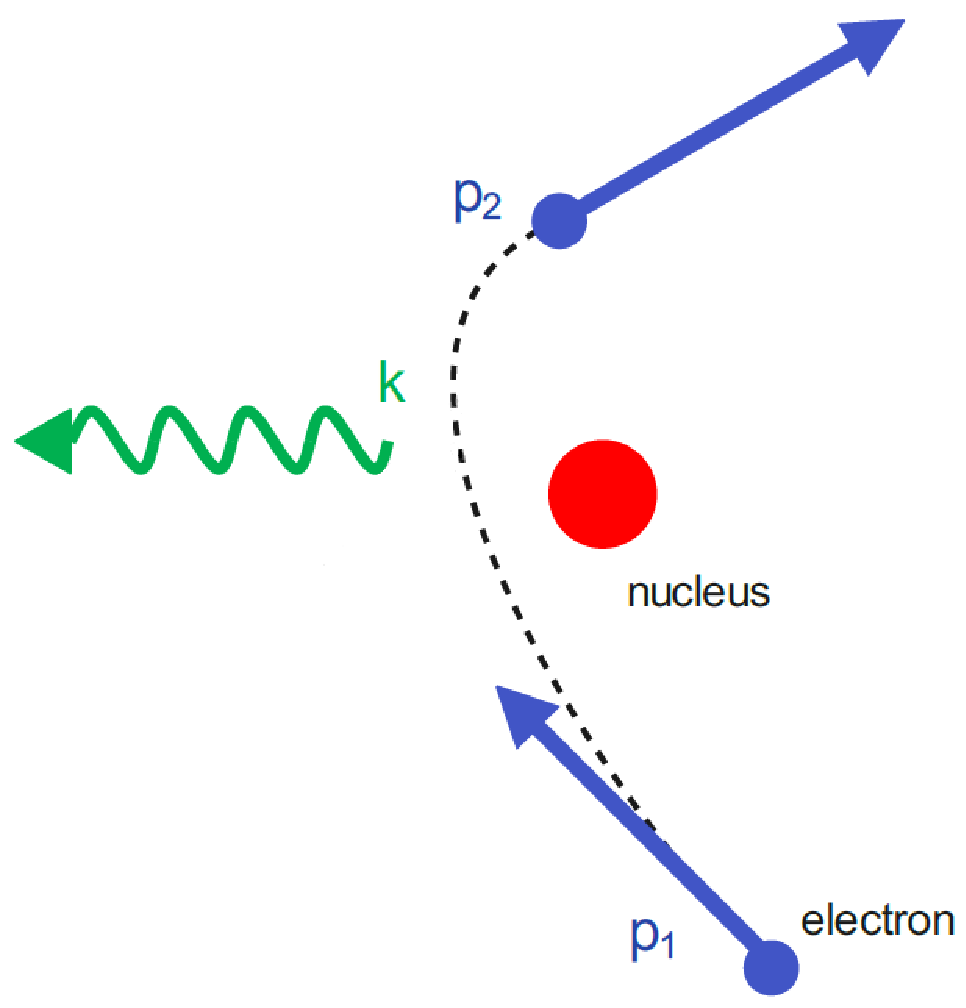
\includegraphics[width=0.5\textwidth]{Figures/DIANA_Inverse_Compton_Source_Design/Bremsstrahlung_fixed.pdf}
\caption{Diagram of the bremsstrahlung process where an electron (blue) with momentum $p_{1}$ is bent from its original trajectory by the Coulomb attraction of a nearby nucleus (red), the momentum of the electron is modified $p_{2}$ and a photon (green) is generated with momentum $\hbar k$, with energy equal to the kinetic energy reduction of the electron.}
\label{fig:bremsstrahlung_diagram}
\end{figure}

The differential cross section of the bremsstrahlung interaction as a function of generated photon energy per unit $m_{e}c^{2}$, $k$ for a thin target is given by Bethe \cite{bethe1934influence,koch1959bremsstrahlung} as 
\begin{multline}
\frac{d\sigma}{dk} = \frac{2Z^{2}r_{e}^{2}}{137k}\left\{\left[1+\left(\frac{E}{E_{0}}\right)^{2}-\frac{2}{3}\frac{E}{E_{0}}\right]\left[\ln{M\left(0\right)}+1-\frac{2}{b}\tan^{-1}\left(b\right) \right] \right.\\\left. +\frac{E}{E_{0}}\left[\frac{2}{b^{2}}\ln\left(1+b^{2}\right)+\frac{4\left(2-b^{2}\right)}{3b^{2}}\tan^{-1}\left(b\right)-\frac{8}{3b^{2}}+\frac{2}{9}\right]\right\},
\label{eq:bremsstrahlung_differential_cross_section}
\end{multline}
where $Z$ is the atomic number of the target (convertor) element, $E_{0}$ is the energy of the incident electron per unit $m_{e}c^{2}$, $E$ is the energy of the outgoing electron per unit $m_{e}c^{2}$, the impact parameter $b$ is given by 
\begin{equation}
b = \frac{2E_{0}EZ^{1/3}}{111k},
\label{eq:b_impact_parameter}    
\end{equation}
and the constant $M\left(0\right)$ \cite{schiff1951energy} is given by the function
\begin{equation}
\frac{1}{M\left(y\right)} = \left(\frac{k}{2E_{0}E}\right)^{2}+\left(\frac{Z^{1/3}}{111\left(y^{2}+1\right)}\right),
\label{eq:M0_Schiff}    
\end{equation}
when $y=0$. The total cross section of the bremsstrahlung interaction, following the results of Koch and Motz \cite{koch1959bremsstrahlung}, is therefore
\begin{equation}
\sigma = \frac{4Z^{2}r_{e}^{2}}{137}\left[\ln\left(183Z^{-1/3}\right)+\frac{1}{18}\right].
\label{eq:brem_total_cross_section}    
\end{equation}
For example, for a tungsten ($Z = 74$) target, the total cross section of the bremsstrahlung reaction is $\sigma = 4.87\times 10^{-27}$~\si{\meter}$^{2}$, a factor $\sim 73$ larger than the Thomson cross section. 

The differential cross section (Eq.~\ref{eq:bremsstrahlung_differential_cross_section}) can then be converted into the intensity of a bremsstrahlung source via a reaction rate scaling factor
\begin{equation}
\Gamma = \frac{\rho\tau N_{A}}{A},
\label{eq:bremsstrahlung_reaction_rate}    
\end{equation}
where $\rho$ is the density of the bremsstrahlung target, $\tau$ is the target thickness, $N_{A}$ is Avogadro's constant and $A$ is the atomic weight of the target isotope. Hence, the intensity of a bremsstrahlung source is given by
\begin{equation}
I = \Gamma\frac{d\sigma}{dk}
\label{eq:bremsstrahlung_intensity}    
\end{equation}
where the intensity of the bremsstrahlung source is quoted in units of number of photons per unit electron per \si{\mega\electronvolt} per \si{\milli\meter} of target (convertor) thickness (ph/($e^{-}$\si{\mega\electronvolt}\si{\milli\meter})).

The differential and total cross sections in (Eq.~\ref{eq:bremsstrahlung_differential_cross_section}) makes several approximations such as the Born approximation, that an approximate screening potential is used, that the angle of the initial momentum of the electron $\theta_{0}$ is approximated as $\theta_{0} \lessim Z^{1/3}/111E_{0}$ and that the generated photon, incident and outgoing electron are all ultra-relativistic ($k,~E_{0},E \gg m_{e}c^{2}$). The Born approximation requires the initial and final velocities of the electron to satisfy the equations
\begin{align}
\frac{2\pi Z}{137\beta} &\ll 1, & \frac{2\pi Z}{137\beta_{0}} &\ll 1,
\label{eq:Born_approximation}    
\end{align}
where $\beta$ and $\beta_{0}$ are the Lorentz speed factors of the outgoing and incident electron. Screening occurs when electrons of the atom limit the attractive Coulomb force of the nucleus and the screening potential is of the form $Ze\exp\left(-r/a\right)$ \cite{schiff1951energy} with $r$ the distance from the interaction (in terms of the Compton wavelength $\lambdabar = \hbar/m_{e}c$) and $a$ the angle of the generated photon with respect to the incident electron beam.

The Born approximation (Eq.~\ref{eq:Born_approximation}) for an ultra-relativistic incident electron ($\beta_{0}\sim 1$) is only valid for low-Z isotopes up to $Z = 22$. Most isotopes selected for bremsstrahlung targets have high-Z as explained later in this section, for example tungsten ($Z = 74$) is a common bremsstrahlung target material. However, even where there is a breakdown of the Born approximation, for example at high-Z, the accuracy of the bremsstrahlung cross section is still reasonable \cite{koch1959bremsstrahlung} and an overestimation of the cross section on the order of 10\% is predicted \cite{olsen1957theory}. The accuracy of the differential cross section (Eq.~\ref{eq:bremsstrahlung_differential_cross_section}) beyond the breakdown of the Born approximation (Eq.~\ref{eq:Born_approximation}) is demonstrated in Fig.~\ref{fig:BremIntensityEZ} via a comparison between the intensity resulting from (Eq.~\ref{eq:bremsstrahlung_intensity}) and the results of a \textsc{GEANT4} \cite{agostinelli2003geant4} for a tungsten ($Z = 74$) target at several ultra-relativistic incident photon energies. \textsc{GEANT4} uses a more sophisticated model including re-absorption of generated photons...\textcolor{blue}{**read GEANT4 manual, add to this and cite here**} to model the bremsstrahlung interaction and provides a more accurate prediction of the bremsstrahlung spectrum than the simple differentical cross section (Eq.~\ref{eq:bremsstrahlung_differential_cross_section}).   
\begin{figure}[!h]
\centering
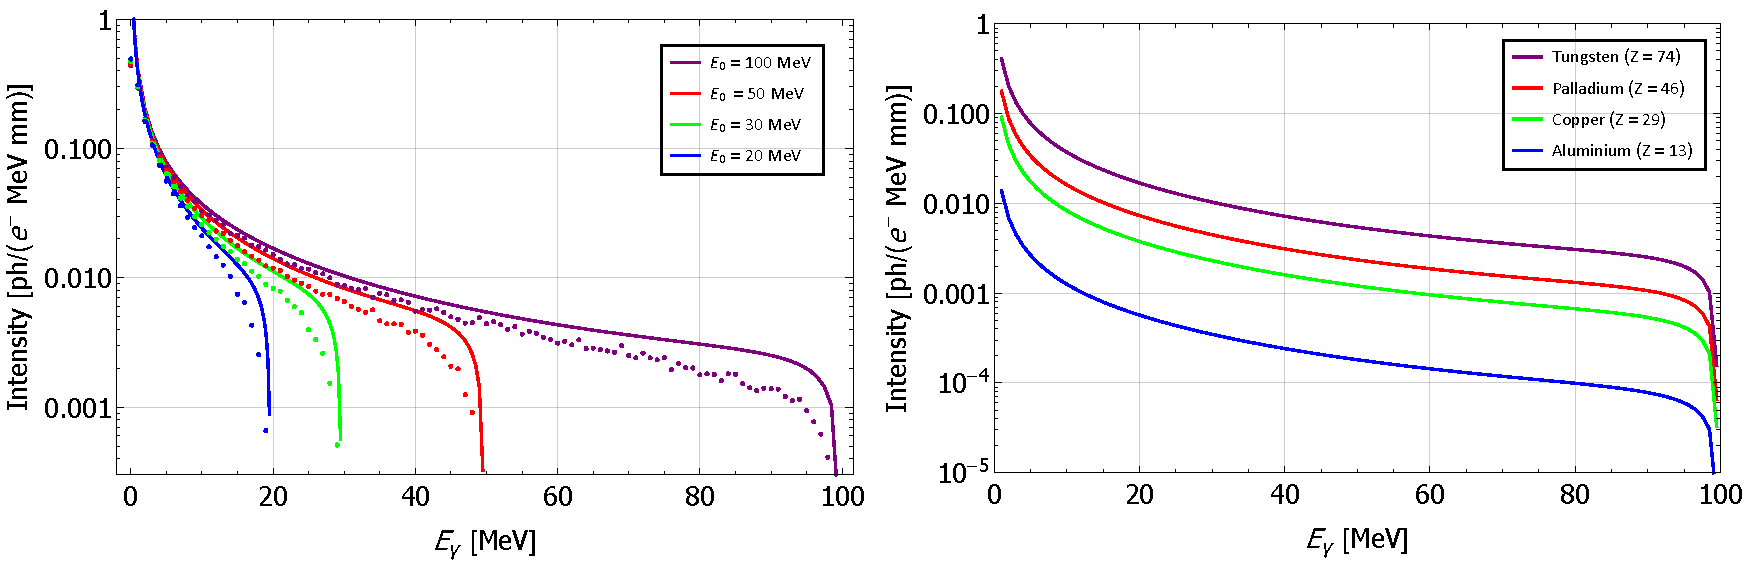
\includegraphics[width=\textwidth]{Figures/DIANA_Inverse_Compton_Source_Design/BremIntensityEZ.pdf}
\caption{Bremsstrahlung generated photon intensity spectra as a function of generated photon energy for several incident photon energies and target materials. Left: Analytical bremsstrahlung generated photon intensity (Eq.~\ref{eq:bremsstrahlung_intensity}) (line) and \textsc{GEANT4} simulated generated photon intensity (point) spectra as a function of generated photon energy for several incident electron energies: 20 (blue), 30 (green), 50 (red) and 100~\si{\megaelectronvolt} (purple) for a tungsten ($Z = 74$) target beyond the breakdown of the Born approximation (Eq.~\ref{eq:Born_approximation}). Agreement between \textsc{GEANT4} and analytical models becomes worse with increasing incident electron energy. Right: Analytical bremsstrahlung generated photon intensity (Eq.~\ref{eq:bremsstrahlung_intensity}) spectrum as a function of generated photon energy assuming a 100~\si{\mega\electronvolt} incident electron for several target materials: tungsten (purple), palladium (red), copper (green), aluminum (blue).}
\label{fig:BremIntensityEZ}
\end{figure}

The bremsstrahlung generated photon intensity spectra produced in Fig.~\ref{fig:BremIntensityEZ} show that a continuous spectrum is produced with photon energies up to a cut-off of $k = E_{0}$ which corresponds to the Duane-Hunt law (Eq.~\ref{eq:Duane_Hunt_law}) where all of the kinetic energy of the incident electron is transferred to the generated photon. The intensity of the generated photon spectrum is largest for the lowest energy photons and decreases with increasing photon energy. Near the maximum generated photon energy ($k = E_{0}$) there is a sharp cut off. 

The differential cross section for bremsstrahlung generation of photons (Eq.~\ref{eq:bremsstrahlung_differential_cross_section}) shows that approximately $d\sigma/dk \propto Z^{2}$, therefore the target (convertor) must be selected with a high atomic number to maximise the number of photons produced. Fig.~\ref{fig:BremIntensityEZ} shows that the highest $Z$ material plotted (tungsten) produces the largest intensity of generated photons. Tungsten ($Z = 74$) is a commonly chosen material because it has high-Z and therefore a large cross section, a high melting point of 3695~\si{\kelvin} as well as a moderate thermal conductivity $\kappa = 174$~\si{\watt}\si{\meter}$^{-1}$\si{\kelvin}$^{-1}$. A high thermal conductivity and melting point are advantageous because bremsstrahlung targets are heated by the incident electron beam so a high melting point allows for a large incident beam power without affecting the target and a high thermal conductivity allows for the heat to be dissipated effectively. 

The number of photons generated is also dependent upon the thickness of the target material as shown in Fig.~\ref{fig:bremsstrahlung_target_thickness} where the bremsstrahlung intensity spectrum is simulated using \textsc{GEANT4} \cite{agostinelli2003geant4} for a 50~\si{\mega\electronvolt} electron beam incident upon a tungsten target of various thicknesses. From the simple reaction rate scaling (Eq.~\ref{eq:bremsstrahlung_reaction_rate}) it would be expected that the number of photons increases linearly with the thickness of the target however, this ignores effects such as the re-absorption of the generated photons within a thick sample. Instead, in Fig.~\ref{fig:bremsstrahlung_target_thickness} we find that there is an optimum target thickness of $\sim 4$~\si{\milli\meter} where the most photons -- $\sim 0.5$ photons in the energy range 10--20~\si{\mega\electronvolt} per electron -- are generated by the bremsstrahlung interaction. This is consistent with the comparative intensity against target thickness plot in Fig.~\ref{fig:bremsstrahlung_target_thickness} which shows a 5~\si{\milli\meter} thick tungsten target produces the most photons.  
\begin{figure}[!h]
\centering
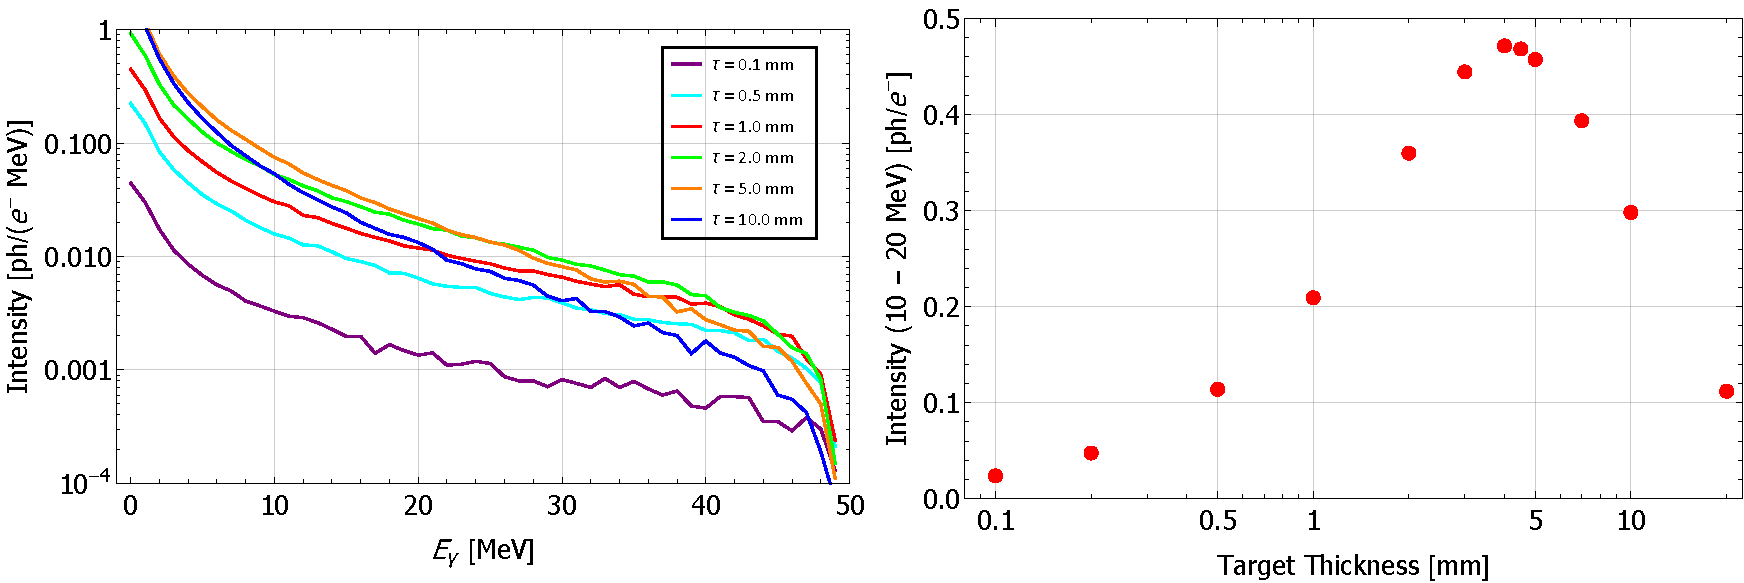
\includegraphics[width=\textwidth]{Figures/DIANA_Inverse_Compton_Source_Design/brem_thickness_studies.pdf}
\caption{Left: \textsc{GEANT4} bremsstrahlung generated photon intensity spectrum as a function of generated photon energy for 50~\si{\mega\electronvolt} electrons incident on a tungsten target of varying thickness: 0.1 (purple), 0.5 (cyan), 1.0 (red), 2.0 (green), 5.0 (orange), 10.0~\si{\milli\meter} (blue). Intensity of generated photons increases until $\tau = 5$~\si{\milli\meter} where re-absorption of generated photons in a thicker target decreases the intensity. Right: Summed intensity from 10--20~\si{\mega\electonvolt} of the \textsc{GEANT4} generated photon bremsstrahlung spectrum as a function of simulated target thickness for a 50~\si{\mega\electronvolt} electron incident upon a tungsten target. Intensity of generated photons increases until a peak of $\tau = 4$~\si{\milli\meter} where re-absorption of photons decreases intensity.}
\label{fig:bremsstrahlung_target_thickness}
\end{figure}

Bremsstrahlung sources are typically more simple to construct than ICS sources since a particle beam need only be incident on a stationary target not a counter propagating laser pulse and are consequently cheaper. As bremsstrahlung generates photons with energies up to maximum kinetic energy of the particle bunch incident on the target due to the Duane-Hunt Law (Eq.~\ref{eq:Duane_Hunt_law}), \si{\mega\electronvolt}-scale photons are available with much lower electron energies. For example, 1~\si{\mega\electronvolt} $\gamma$-rays can be produced by inverse Compton scattering via an interaction of an Nd:YAG ($\lambda = 1064$~\si{\nao\meter}) incident laser and a $\sim 235$~\si{\mega\electronvolt} electron bunch in comparison to a bremsstrahlung source where 1~\si{\mega\electronvolt} $\gamma$-rays are readily available from a 5--10~\si{\mega\electronvolt} electron bunch incident on a tungsten target. Therefore, \si{\mega\electronvolt}-scale photons from a bremsstrahlung source can be produced by a small accelerator using only a converter target and an electron
accelerator \cite{chin2021application}, whereas a larger electron accelerator is required for an ICS source operating at similar energies.

However, unlike the ICS process there is no inherent photon energy--angle correspondence in bremsstrahlung sources, therefore energies of photons can not be simply selected by a collimator. In bremsstrahlung sources photon energy selection is not readily achievable; the spectrum may be narrowed by attenuating the bremsstrahlung photons through a material as lower energy photons would be attenuated to a greater extent than the higher energy photons, but some would still remain and the attenuation would distort the spectrum overall whilst reducing photon fluxes. Therefore, attenuation of the spectrum is a poor way of obtaining a monochromatic photon spectrum. Unavoidably bremsstrahlung $\gamma$-ray sources produce photons with a broad energy range, as shown in Fig.~\ref{fig:BremIntensityEZ} that delivers unnecessary dose to a sample which can also interfere with the signature to be detected \cite{geddes2017impact}. Broadband radiation reduces the signal-to-noise ratio of the investigated process, consequently monoenergetic sources allow the sensitivity of a experiment to be improved \cite{jones2008bremsstrahlung}.

To compare the DIANA ICS source with a common bremsstrahlung source we consider a 1~\si{\milli\ampere} electron beam from an electron linac with a maximum electron beam energy of 50~\si{\mega\electronvolt}, similar to the demonstrated 0.85~\si{\milli\ampere} ELBE linac \cite{teichert2003results}, is incident on a 1~\si{\milli\meter} thick tungsten ($Z = 74$) target. The resultant spectrum in terms of spectral density (ph/(MeV s)) using the analytical bremsstrahlung intensity  (Eq.~\ref{eq:bremsstrahlung_intensity}) at a current of 1~\si{\milli\ampere} is given in Fig.~\ref{fig:brem_1mA_DIANA_ICS_comparison}. The DIANA ICS source spectrum at $E_{\gamma} = 20$~\si{\mega\electronvolt} is selected as a comparison and the spectrum in Fig.~\ref{fig:DIANA_spectra} has been scaled by the 12.5~\si{\milli\ampere} current of the DIANA ERL for conversion from a single electron bunch--laser pulse interaction spectrum to the ICS interaction spectrum per second.
\begin{figure}[!h]
\centering
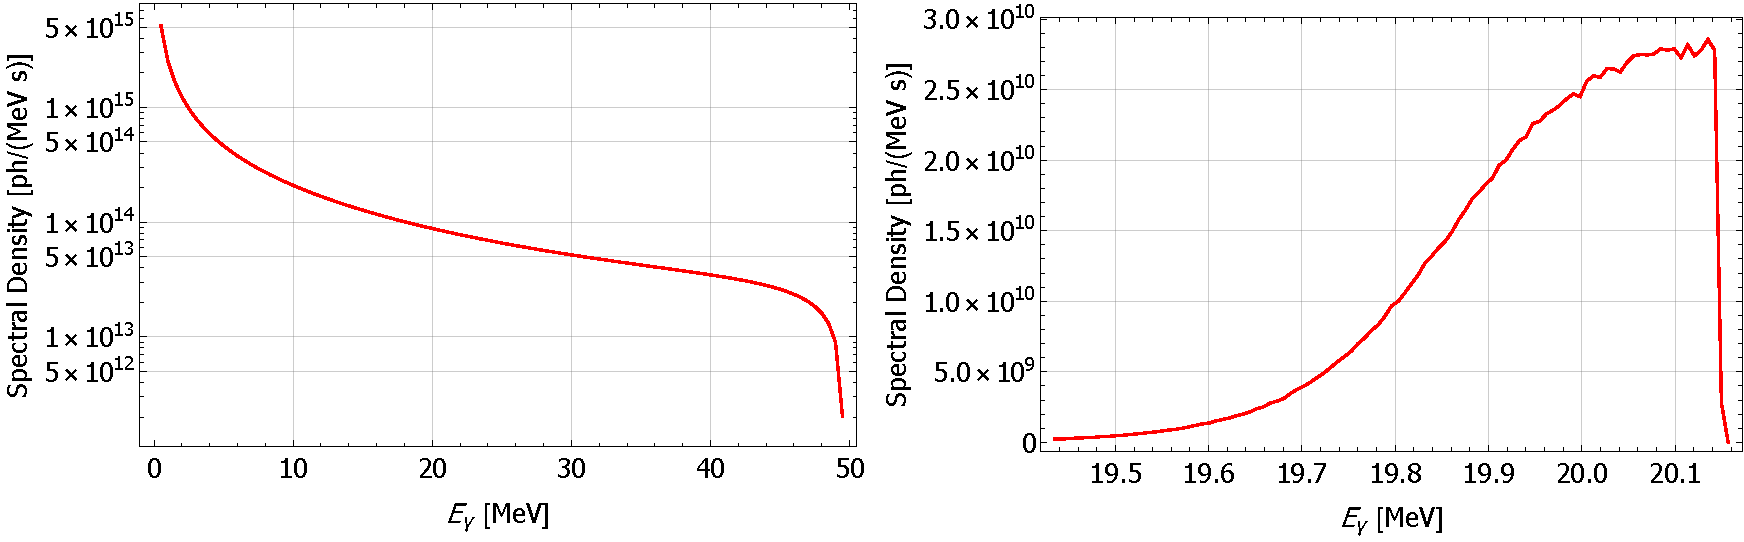
\includegraphics[width=\textwidth]{Figures/DIANA_Inverse_Compton_Source_Design/Brem_1mA_DIANA_ICS_Comparison.pdf}
\caption{Left: Analytical generated photon bremsstrahlung spectrum for 50~\si{\mega\electonvolt} electrons at a current of 1~\si{\milli\ampere} incident upon a 1~\si{\milli\meter} thick tungsten target (convertor). Right: DIANA ICS source scattered photon produced using \textsc{ICARUS} for a the interaction of a 1072~\si{\mega\electronvolt} electron beam with a 12.5~\si{\milli\ampere} average beam current and a Nd:YAG laser ($\lambda=1064$~\si{\nano\meter}) at a 5\si{\degree} crossing angle. This spectrum is scaled from the single interaction spectrum in Fig.~\ref{fig:DIANA_spectra} for the photons generated from the DIANA ICS source within one second.}
\label{fig:brem_1mA_DIANA_ICS_comparison}
\end{figure}
The 1~\si{\milli\ampere}, 50~\si{\mega\electronvolt} bremsstrahlung source produces a total flux of $\mathcal{F} = 9.94\times 10^{15}$~ph/\si{\second}, which is much larger than the total flux ($\mathcal{F} = 6.08\times 10^{10}$~ph/\si{\second}) of the DIANA ICS source configured for $E_{\gamma} = 20.11~\si{\mega\electronvolt}$ because the bremsstrahlung cross section is much larger than the ICS cross section ($\sigma_{Z = 74} \sim 73\sigma_{T}$) and the number of nuclei present in the tungsten target is much larger than the number of photons in the laser pulse. The number of photons produced within the scattered photon energy range of the DIANA ICS spectrum ($19.44~\mathrm{\si{\mega\electronvolt}} \leq E_{\gamma} \leq 20.16~\mathrm{\si{\mega\electronvolt}}$) is $1.29\times 10^{9}$~ph/\si{\second}, as shown in Table~\ref{tab:DIANA_spectral_output}, however the bremsstrahlung source over the same generated photon energy range ($19.44~\mathrm{\si{\mega\electronvolt}} \leq E_{\gamma} \leq 20.16~\mathrm{\si{\mega\electronvolt}}$) produces $6.44\times 10^{13}$~ph/\si{\second} -- a factor $4.99\times 10^{4}$ the flux in a 0.5\% \textit{rms} BW of the DIANA ICS source. Therefore, we can conclude that conventional bremsstrahlung sources exceed ICS sources in terms of flux. However, bremsstrahlung sources are inherently broadband with a continuous spectrum and do not allow for photons of particular energies to be selected unlike ICS sources.

%The ARIEL project at TRIUMF \cite{dilling2013ariel} is an example of a dedicated high flux bremsstrahlung source, where electron bunches from a linear accelerator are incident on a 8~\si{\milli\meter} thick lead (Z=82) target \cite{lebois2011simulations}. The ARIEL linac produces electron bunches with electron beam energies up to 50~\si{\mega\electronvolt} and produces a CW average electron beam current of 10~\si{\milli\ampere} \cite{dilling2013ariel}, resulting in an average electron beam power of 500~\si{\kilo\watt} incident on the lead target. The bremsstrahlung interaction is expected to produce a total flux of $10^{11}$--$10^{14}$~ph/\si{\second} \cite{lebois2011simulations}, which is four orders of magnitude higher than the flux of DIANA ICS source in Table~\ref{tab:DIANA_spectral_output}. Therefore, conventional bremsstrahlung sources typically produce higher flux than ICS sources though this is over a large range of photon energies. 

Laser plasma wakefield accelerators \cite{sprangle1988laser,esarey2009physics}, have also been considered for compact (small accelerator footprint) bremsstrahlung generation of $\gamma$-rays \cite{cipiccia2012tuneable,lemos2018bremsstrahlung}. A discussion of laser wakefield acceleration is not included here, but a discussion is presented by Esarey et al \cite{esarey2009physics}. Cipiccia et al \cite{cipiccia2012tuneable} used a Ti:Sa laser ($\lambda = 800$~\si{\nano\meter}) with pulse energy 2.5--3.5~\si{\joule} and laser pulse duration 60--80~\si{\femto\seconds} FWHM to generate 20--25~\si{\pico\coulomb} electron bunches with energies in the range 200--400~\si{\mega\electronvolt} and an \textit{rms} energy spread of 8\%. The 20--25~\si{\pico\coulomb} electron bunches were incident upon a 2~\si{\centi\meter} aluminium ($Z=13$) target generating $1\times 10^{9}$ bremsstrahlung photons with photon energies up to $\sim 220$~\si{\mega\electronvolt} and a mean energy of 10~\si{\mega\electronvolt}. A photon flux of $1\times 10^{9}$~ph/\si{\second} is a factor of $\sim 61$ smaller than the flux of the DIANA ICS source in Table~\ref{tab:DIANA_spectral_output}, therefore LWFA bremsstrahlung sources are incapable of the high flux of conventional sources such as the 1~\si{\milli\ampere} electron linac bremsstrahlung source and the proposed DIANA ICS source. The high flux in a narrow bandwidth ($\mathcal{F}_{\mathrm{0.5\%}} = 1.30\times 10^{9}$~ph/\si{\second}, 0.5\% \textit{rms} bandwidth) achievable from DIANA is far beyond what is available at LWFA bremsstrahlung sources.    

\section{DIANA ICS Applications}
\label{sec:DIANA_ICS_applications}
% Say only certain examples chosen, not comprehensive

A series of ICS sources driven by DIANA would enable a broad range of experiments within nuclear photonics \cite{nedorezov2017nuclear,budker2021expanding} and nuclear physics more broadly, such as nuclear resonance fluorescence (NRF), transmutation of waste, nuclear forensics and security, as well as fundamental nuclear physics such as photonuclear cross section measurements \cite{renstrom2018verification}.
More broadly, experiments can be performed in fields such as high energy astrophysics, high energy physics and fundamental tests of quantum mechanics, as well as medical isotope production. The DIANA ICS source, with spectral output parameters shown in Table~\ref{tab:DIANA_spectral_output}, offers high flux and a narrow bandwidth which are required for experimentation in these areas, and allows for greater precision measurement than previous sources, as discussed in Sections~\ref{sec:gamma_ICS_comparison} and~\ref{sec:bremsstrahlung_comparison}. The preliminary examination of applications for the DIANA ICS has focused upon nuclear resonance fluorescence, transmutation of radioactive wastes and photonuclear medical isotope production -- areas in which a high average brilliance, narrowband $\gamma$-ray source can excel.  

\subsection{Nuclear Resonance Fluorescence}

Nuclear resonance fluorescence is a process first described by Kneissl et al \cite{kneissl1996investigation} where a nucleus of an atom resonantly absorbs a $\gamma$-ray, exciting the nucleus to a higher energy excited state; the nucleus subsequently decays via emission of a $\gamma$-ray to a lower energy state. Applied to a bulk sample, with a beam of $\gamma$-rays, the $\gamma$-rays emitted via NRF are distributed isotropically (i.e. uniform angular distribution) and the energy of the $\gamma$-rays is characteristic of the particular isotope that is being resonantly excited, therefore NRF is applicable to isotopic determination of samples. Nuclear resonance fluorescence is the nuclear (isotopic) analog of x-ray resonance fluorescence (as described in Section~\ref{sec:CBETA_ICS_applications}) used for atomic (elemental) discrimination of samples. Specific measurement methods are explained later in this section. 

Nuclear resonance fluorescence was initially applied to the detection of nuclear materials for security purposes such as the detection of clandestine nuclear material \cite{bertozzi2005nuclear,pruet2006detecting,geddes2017impact} for non-proliferation, then subsequently applied to the assay and identification of nuclear waste \cite{hayakawa2010nondestructive,angell2015demonstration,bolind2015states} and for imaging of manufacturing defects in reactor fuel. Both bremsstrahlung \cite{bertozzi2005nuclear} and inverse Compton scattering sources \cite{angell2015demonstration} of $\gamma$-rays have been utilised to provide the incident $\gamma$-ray beam for NRF experimentation. Angell et al \cite{angell2015demonstration} have demonstrated an NRF measurement of an aluminium proxy target inside a radioactive waste canister using the HI$\gamma$S ICS source with a 3.7\% error on the expected value (within the expected 7\% experimental error). Large experimental errors occurred because of the 3.7\% FWHM bandwidth of the HI$\gamma$S ICS source and because of limitations in the determining the flux of the ICS source. A schematic diagram of a NRF experiment utilising an ICS source is shown in Fig.~\ref{fig:NRF_diagram}.
\begin{figure}[!h]
\centering
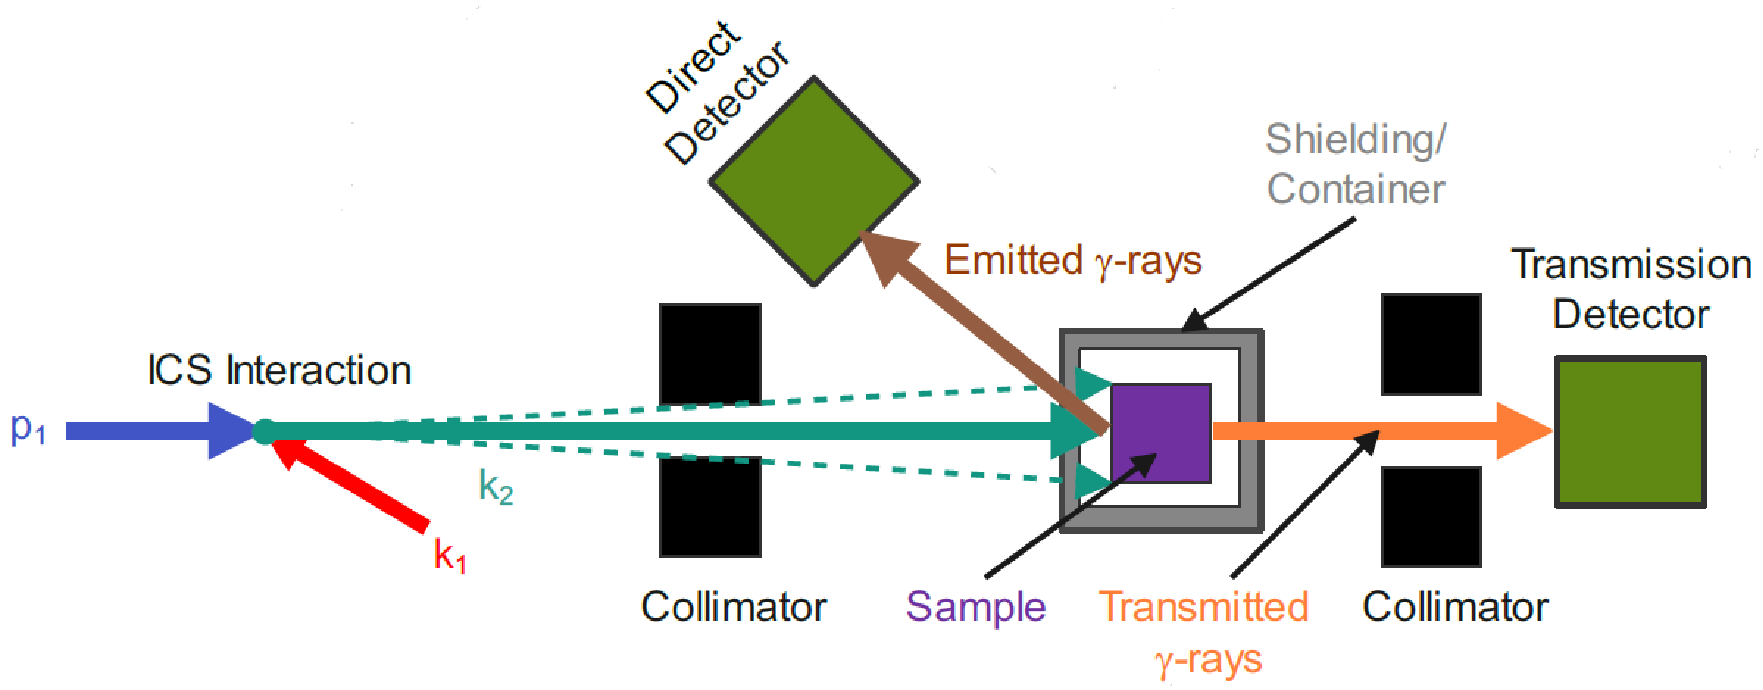
\includegraphics[width=\textwidth]{Figures/DIANA_Inverse_Compton_Source_Design/NRF_diagram_fixed.pdf}
\caption{Diagram of a nuclear resonance fluorescence experiment using a $\gamma$-ray beam (turquoise) generated by an ICS source. A relativistic electron bunch (blue) of momentum $p_{1}$ is interacted with an incident photon pulse (red) of momentum $\hbar k_{1}$ to scatter a $\gamma$-ray photon beam of momentum $\hbar k_{2}$, which is collimated (black) for narrow bandwidth and passed through a shielded (grey) sample (purple).  For transmission measurements the $\gamma$-ray beam is detected by a downstream on-axis detector, after photons are absorbed by the sample at the resonant excitation energies. Direct measurements are conducted by sampling the $\gamma$-rays emitted from the sample from the de-excited states by an off-axis detector.}
\label{fig:NRF_diagram}
\end{figure}

The intrinsic resonance width of an excited state in the nucleus is of the order \si{\milli\electronvolt} to \si{\electronvolt}, and is further broadened to several \si{\electronvolt} by Doppler broadening \cite{angell2015demonstration}, which occurs due to the thermal motion of the nuclei in the target material. Therefore, direct probing of just the resonance width would require a $\gamma$-ray beam probe with energy spread on the order of several electronvolts which, with resonances excited on the \si{\mega\electronvolt}-scale, would require a bandwidth on the order of $\Delta E_{\gamma}/E_{\gamma} = 10^{-6}$. Production of $\gamma$-rays with bandwidth on the $10^{-6}$ scale has only been demonstrated using $\gamma$-rays from radioactive sources, which lack the required flux for short timescale measurements

A single nuclear resonance may be probed if the energy spread of the $\gamma$-ray pulse is smaller than the energy variation between its nearest-neighbour resonances. For example, consider the three lowest (and closest in excitation energy) measured excited states of uranium-238, where resonances can be excited with 2.176~\si{\mega\electronvolt}, 2.209~\si{\mega\electronvolt} and 2.245~\si{\mega\electronvolt} $\gamma$-rays respectively \cite{quiter2011transmission}. A $\gamma$-ray beam probe may excite just the 2.209~\si{\mega\electronvolt} resonance if the $\gamma$-ray has a central energy of 2.209~\si{\mega\electronvolt} and the total energy spread of the $\gamma$-ray beam is less than $\Delta E_{\gamma} = 33$~\si{\kilo\electronvolt} (a FWHM value of 25.9~\si{\kilo\electronvolt}) and therefore the FWHM bandwidth of the $\gamma$-ray beam must be $\Delta E_{\gamma}/E_{\gamma} = 0.0117$ i.e a 1.17\% FWHM (0.5\% \textit{rms}) bandwidth. In mixtures of radioisotopes, such as in unknown nuclear waste repositories, the analysis becomes more complex with more and unknown resonances present. 

Bremsstrahlung has a continuous spectrum, as shown in Section~\ref{sec:bremsstrahlung_comparison}, therefore single nuclear resonances may not be probed and the spectrum of emitted radiation from the NRF assayed sample will have multiple radiation peaks, which are more challenging to discriminate -- especially in poly-isotopic samples. Whilst bremsstrahlung NRF detection methods are feasible, the associated measurement error is larger than for ICS sources because more background radiation is produced \cite{angell2015demonstration}. However, ICS sources such as DIANA are capable of narrow bandwidth $\gamma$-ray beam generation and can therefore be used to target single resonances, therefore ICS sources are more suited to NRF experiments.  

Measurements of samples via NRF can be conducted using two methods: transmission and direct, as shown in Fig.~\ref{fig:NRF_diagram}. Direct measurement involves a detector placed at an angle off-axis from the $\gamma$-ray beam, and measures the isotropically emitted $\gamma$-rays from the decaying excited states. Sample material can be identified with the use of reference isotopes, or reference spectra and quantification of the material is achieved similarly via comparison of the intensity of the emitted $\gamma$-rays with reference material \cite{angell2015demonstration}. Transmission measurements place the detector on-axis, measuring the incident $\gamma$-rays that pass through the sample, $\gamma$-rays with energies at the excitation energies of the sample nuclei are absorbed, leaving notches in the measured spectrum. The energies of the notches allow for identification of the sample material and the depth of the notches, in comparison to reference material, allows for quantification \cite{pruet2006detecting}. Transmission measurements are typically quicker as the full absorption of $\gamma$-rays is measured whereas in a direct measurement only a smaller solid angle of the emitted photons are collected, so only part of the emission (and therefore absorption) is measured, hence transmission measurements are generally preferred.

The first nominal electron energy ($E_{e} = 362$~\si{\mega\electronvolt}) of the DIANA ICS source is capable of producing tunable $\gamma$-rays with a centre energy of 2.33~\si{\mega\electronvolt}, which is useful for nuclear resonance fluorescence based assays of fissile materials; fissile materials have strongly excited energy levels at 2--3~\si{\mega\electronvolt} \cite{angell2015demonstration}. Strongly excited levels occur at 2--3~\si{\mega\electronvolt} in isotopes such as uranium because of the scissor modes of nuclei \cite{iudice1978new,bohle1984new} -- where, in a deformed nucleus, the protons and neutrons oscillate out of plane to each other. Comparatively, a high flux ICS source such as DIANA would also be useful in reducing the measurement time (proportional to the number of incident $\gamma$-rays) of NRF studies over demonstrated ICS sources as the flux of DIANA is 110 times larger than HI$\gamma$S \cite{weller2009research}.

The three isotopes of high importance in nuclear proliferation are $^{238}\mathrm{U}$, $^{235}\mathrm{U}$ and $^{239}\mathrm{Pu}$, which have resonances for incident photon energies at $E_{238~U}^{\mathrm{NRF}} = 2.176$~\si{\mega\electronvolt} \cite{quiter2011transmission},  $E_{235~U}^{\mathrm{NRF}} = 1.733$~\si{\mega\electronvolt} and  $E_{239~Pu}^{\mathrm{NRF}} = 2.143$~\si{\mega\electronvolt} \cite{hayakawa2010nondestructive}. Tuning the electron bunch energy of DIANA in the first turn within the electron energy range $E_{\gamma} =$ 312--350~\si{\mega\electronvolt} allows NRF studies of these isotopes. Using a similar comparison to that employed for spacing between uranium-238 resonances, we see that the difference between $^{238}\mathrm{U}$ \cite{quiter2011transmission} and $^{239}\mathrm{Pu}$ \cite{hayakawa2010nondestructive} resonances is often on the order of $\sim$10--100~\si{\kilo\electronvolt} -- resolvable with the DIANA ICS source. Therefore, a narrowband source with tunability of both the scattered photon energy (Eq.,~\ref{eq:scattered_photon_energy}) and the bandwidth of the $\gamma$-ray beam (Eq.~\ref{eq:RMS_bandwidth}) is a requirement for isotopic determination by NRF.

In addition, collective modes of nuclei such as giant dipole resonances \cite{goldhaber1948nuclear,baldwin1947photo}, pygmy dipole resonances \cite{cook1957photodisintegration,tonchev2010spectral} and scissor modes \cite{iudice1978new,de1984reformulation,bohle1984new} can be probed via NRF techniques using $\gamma$-ray ICS sources. Collective modes of nuclei study the oscillations of the nucleons within a nucleus, for example giant dipole resonances occur when the protons and neutrons in a nucleus oscillate around their equilibrium positions with respect to each other forming an electric dipole mode. Excitation of these collective modes can be of use in nuclear structure studies.

An example of NRF studies of collective modes of nuclei is the study of the M1 scissors mode of a $^{152}\textrm{Sm}$ nucleus, which has recently been probed at the HI$\gamma$S source to investigate the electric quadrupole (E2) mode decay \cite{ide20212}. However, this experiment was limited by the large 100~\si{\kilo\electronvolt} FWHM bandwidth ($\gamma$-ray energy spread) \cite{ide20212} of the source at the $E_{\gamma} = 2.995$~\si{\mega\electronvolt} incident $\gamma$-ray energy required to probe the scissor mode \cite{ziegler1993low} and consequently excited states beyond the $2^{+}$ state are inaccessible because of the insensitivity of the incident $\gamma$-ray beam \cite{ide20212}. However, the DIANA ERL ICS source using a 362~\si{\mega\electronvolt} electron bunch ($E_{\gamma} =$ 2.33~\si{\mega\electronvolt}) produces a $\gamma$-ray beam with a FWHM energy spread of 25.9~\si{\kilo\electronvolt} -- a factor $\sim4$ smaller than the HI$\gamma$S bandwidth. Therefore, higher precision nuclear physics experiments may be available with the DIANA ICS source. The DIANA ICS source is also designed to produce comparatively larger flux than HI$\gamma$S, as seen in Table~\ref{tab:gammaray_ICS_comparison}, which will improve data acquisition times for these measurements. Improvements in flux and bandwidth with respect to HI$\gamma$S \cite{weller2009research} in DIANA may also be available in ELI-NP-VEGA \cite{elinp2019vega}, where the ELIADE research programme aims to distinguish and separate different excitations in the overlapping region of the pygmy dipole resonance (PDR), the giant dipole resonance (GDR), the magnetic dipole resonance (MDR), and the pygmy quadrupole resonance (PQR) \cite{tanaka2020current}. Experiments in these fields would therefore also be suitable for the DIANA ICS source.

\subsection{Transmutation of Nuclear Waste}

Photonuclear reactions such as $(\gamma,p)$, $(\gamma,n)$, $(\gamma,\alpha)$, $(\gamma,f)$ become possible above $\sim5$~\si{\mega\electronvolt} and are useful for transmutation of isotopes which, when driven by large fluxes of photons, could potentially transform long-lived wastes such as $^{241}\mathrm{Am}$ and $^{129}\mathrm{I}$ \cite{cho2016reconsideration} into wastes with shorter lifespan or otherwise easier to handle. Nuclear transmutation is possible using DIANA as the 2nd ($E_{e}=717$~\si{\mega\electronvolt}, $E_{\gamma}=9.06$~\si{\mega\electronvolt}) and 3rd turn ($E_{e}=1072~\si{\mega\electronvolt}$, $E_{\gamma}=20.11$~\si{\mega\electronvolt}), with spectral output parameters shown in Table~\ref{tab:DIANA_spectral_output}, are capable of producing a high flux of $\gamma$-rays around and above the $\sim10$~\si{\mega\electronvolt} scattered photon energy threshold.

As a case study iodine-129 is investigated, $^{129}\mathrm{I}$ is a major long-lived reactor waste with half-life $T_{1/2} = 1.57\times 10^{8}$~yr, which poses an additional challenge to repository storage methods -- where radioactive waste is shielded and stored for many years -- due to its water solubility \cite{cho2016reconsideration}. Whilst other storage methods are being developed, such as storing the waste in a glass matrix  \cite{lee2021chemical,morizet2021immobilization}, another solution would be transmutation of this waste to a stable state. Rehman et al \cite{ur2017optimization} propose using a giant dipole resonance photonuclear reaction ($\gamma$,n)
\begin{equation}
^{129}\mathrm{I} \left(T_{1/2}=1.57\times 10^{7}\textrm{yr}\right) \xrightarrow[]{\left(\gamma,n\right)} {}^{128}\mathrm{I} \left(T_{1/2}=24.99~\mathrm{\si{\minute}}\right) \substack{\xrightarrow[]{\left(\beta^{-},93.1\%\right)} {}^{128}\mathrm{Xe}~\left(\mathrm{stable}\right)\\[0.1em] \xrightarrow[]{\left(\beta^{+},6.9\%\right)} {}^{128}\mathrm{Te}~\left(\mathrm{stable}\right)}
\label{eq:129I_photonuclear_transmutation}
\end{equation}
where $^{129}\mathrm{I}$ is transmuted to two stable isotopes $^{128}\mathrm{Xe}$ and $^{128}\mathrm{Te}$. The xenon and tellurium isotopes do not require any special handling, and the iodine-129 long-lived waste has been eliminated without any further challenges for repository storage. A similar approach is applicable to many other fission products.

Based on the cross section measurements for $^{129}\mathrm{I}$ by Magill et al \cite{magill2003laser}, as re-created in Fig~\ref{fig:I129_cross_section_photon_energy} using data from the EXFOR database entry \cite{zerkin2018experimental}, the peak cross section of the photonuclear reaction is $\sigma_{\mathrm{reac}} = 229$~\si{\milli\barn} at 15~\si{\mega\electronvolt}. Therefore, 15~\si{\mega\electronvolt} photons would be required to resonantly excite the giant dipole resonance and cause the photonuclear transmutation reaction (Eq.~\ref{eq:129I_photonuclear_transmutation}). Tuning DIANA to the required 15~\si{\mega\electronvolt} scattered photon energy would produce a total of $6.04\time 10^{10}$~ph/\si{\second}, below the $10^{13}$~ph/\si{\second} flux assumed in Rehman et al's \cite{ur2017optimization} calculations. A transmutation rate can be approximated by scaling the transmutation rate with the decrease in flux from Rehman et al's assumed flux ($\mathcal{F}=10^{13}$~ph/\si{\second}), yielding a transmutation rate of $\sim10^{8}$~atoms/\si{\second}. Therefore, only miniscule amounts ($\sim0.1$~\si{\micro\gram}) of iodine 129 could be processed within a year by this method using the DIANA ICS source, but there is scope for proof of principle experiments.
\begin{figure}[!h]
\centering
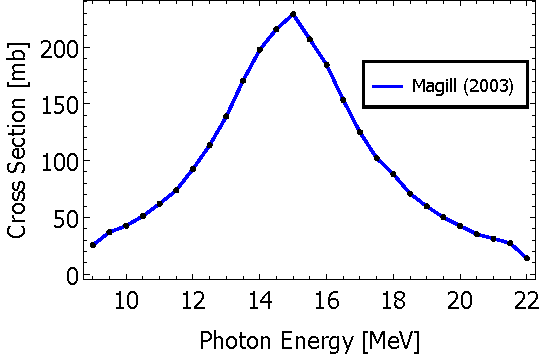
\includegraphics[width=0.7\textwidth]{Figures/DIANA_Inverse_Compton_Source_Design/Iodine_129_cs_photon_energy.pdf}
\caption{Measured \cite{magill2003laser} photonuclear GDR $\left(\gamma,n\right)$ cross section as a function of incident photon energy for the long-lived radioactive waste isotope $^{129}\mathrm{I}$. The cross section peaks at $E_{\gamma} = 15$~\si{\mega\electronvolt} incident photon energy with a cross section of $\sigma = 229$~\si{\milli\barn}. Data acquired from EXFOR database \cite{zerkin2018experimental}.}
\label{fig:I129_cross_section_photon_energy}
\end{figure}

% Further complication by many isotope mixtures
Transmutation of isotopes is further complicated, as waste is often not monoisotopic and other isotopes present in the waste may have similar photonuclear cross sections as a function of photon energy. If the cross sections as a function of energy overlap then that reaction would occur simultaneously with the iodine 129 photonuclear reaction (Eq.~\ref{eq:129I_photonuclear_transmutation}), however the unintended  reaction may cause further issues for waste storage. Therefore, the waste should be properly assayed, for example using NRF, before transmutation is attempted and the photonuclear ($\gamma$,n) reaction cross sections of other long lived wastes present in the sample must be accommodated. Many long-lived reactor wastes, such as palladium-107 and tin-126, require photonuclear cross section measurements as data on these is not available \cite{zerkin2018experimental}. 

\subsection{Photonuclear Medical Isotope Production}
\label{sec:photonuclear_medical_isotope_production}

Radionuclides have abundant uses within medical treatment with applications in imaging, such as $\beta^{+}$ emitting isotopes like $^{18}\mathrm{F}$ ($T_{1/2}=1.83$~\si{\hour}, $\beta^{+}$, 100\%) for use in positron emission tomography (PET) for metabolic uptake studies of tumors \cite{orlhac2014tumor}, and in treatment, such as prostate cancer brachytherapy \cite{yuan2021proof} with $^{192}\textrm{Ir}$ ($T_{1/2} =73.83$~\si{\day}, $\beta^{-}$, 95.13\%, $\epsilon$, 4.87\%). Theranostic \cite{svenson2013theranostics} radionuclide treatments, where isotopes (or combinations of isotopes of the same element) can be jointly used for imagining and treatment, have became a recent focus in this area of research. For example, $^{64}\mathrm{Cu}$ is a theranostic isotope which decays through $\beta^{+}$ (61\%) and $\beta^{-}$ (39\%) routes with the emission of Auger electrons \cite{boschi2018emerging}; allowing simultaneous diagnostic imaging and therapy with the same radio-pharmaceutical.

A range of production methods for medical isotopes are available such as proton cyclotron based production  with $\left(p,x\right)$ reactions, for example for technetium-99m production \cite{gagnon2011cyclotron}, research reactor (neutron irradiation) production with $\left(n,x\right)$ reactions, such as the MURR reactor \cite{ma1996production}, isotope separation on-line (ISOL) production with  proton based photofission $\left(p,f\right)$ reactions -- recently demonstrated for the theranostic terbium quadruplet \cite{muller2012unique} at the MEDICIS facility \cite{dos2014cern} (thought not widely demonstrated clinically) -- as well as the photonuclear production methods with $\left(\gamma,x\right)$ reactions \cite{habs2011production}. Production of medical isotopes typically uses a large flux of particles such as neutrons (research reactor), protons (cyclotrons/ISOL) or photons (photonuclear) incident on a target, which can be mono-isotopic, a natural element (many isotopes) or a compound, to cause favourable particle-induced nuclear reactions such as proton irradiation $\left(p,x\right)$ (cyclotron), neutron irradiation $\left(n,x\right)$ or photonuclear reaction $\left(\gamma,x\right)$. A diagram of a typical medical isotope production experiment using the photonuclear ($\gamma$,n)is shown in Fig.~\ref{fig:isotope_production_diagram}. The resultant products are usually then chemically separated from the target, or separated by mass spectrometer in the case of ISOL \cite{catherall2017isolde} and the produced radioisotope is labelled with a tracer, such as DOTA-folate conjugate cm-09 for $^{44}\mathrm{Sc}$ \cite{muller2013folate}, to be used as the injected radio-pharmaceutical.  
\begin{figure}[!h]
\centering
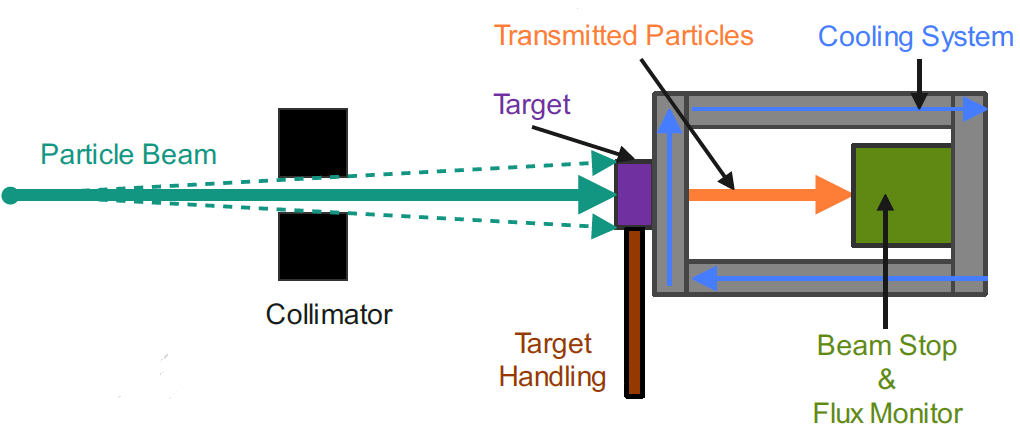
\includegraphics[width=0.8\textwidth]{Figures/DIANA_Inverse_Compton_Source_Design/Isotope_Production_diagram_fixed.png}
\caption{Diagram of a typical photonuclear radioisotope production facility. The particle (photon) beam (turquoise) is collimated (black) then is incident upon a target (purple), which is cooled (blue) for high incident power, and the radio-isotope is produced in the target. The remaining (non-interacted) incident particle beam (orange) then passes through the target and is collected by a beam stop or flux monitor (green). Typically other production methods use similar setups with a flux of irradiating particles incident on a target.}
\label{fig:isotope_production_diagram}
\end{figure}

Due to the unavailability of certain target materials -- as some isotopes don't exist in nature -- some isotopes may only be produced via a few of the methods previously described. For example, the PET imaging radioisotope $^{44}\mathrm{Sc}~\left(T_{1/2}=3.97~\si{\hour}, \beta^{+}, 100\%\right)$\cite{roesch2012scandium,muller2014promising} can be produced via a proton cyclotron by 
\begin{align}
^{45}\mathrm{Ca}&\xrightarrow[]{\left(p,n\right)}{}^{44}\mathrm{Sc},
\label{eq:44Sc_direct} \\
^{45}\mathrm{Sc}&\xrightarrow[]{\left(p,2n\right)}{}^{44}\mathrm{Ti}\left(T_{1/2}=60.25~\mathrm{yr}\right)\xrightarrow[]{\left(\epsilon, 100\%\right)}{}^{44}\mathrm{Sc},
\label{eq:44Sc_generator}
\end{align}
and via a photonuclear method by
\begin{equation}
^{45}\mathrm{Sc}\xrightarrow[]{\left(\gamma,n\right)}{}^{44}\mathrm{Sc}. \label{eq:44Sc_photonuclear}   
\end{equation}

The activity of the sample is also a consideration. For example, imaging radioisotopes (such as PET imagining isotopes like $^{18}$F) must be produced with high enough activity to produce a detectable $\gamma$-ray signal from the patient with good signal-to-noise ratio. For treatment isotopes activity must be high enough to deliver suitable does to the patient. Specific activity of a radioisotope is used to quantify the activity of a produced radioisotopic sample assuming that a pure radioisotope (without admixture of stable isotopes \cite{habs2011production}) is produced and that other contaminating reactions do not interfere during irradiation. The resultant specific activity ($A/m$) in \si{\becquerel}/\si{\milli\gram} of a produced radioisotope at irradiation time $t_{\mathrm{irr}}$ is given by \cite{habs2011production}
\begin{equation}
\frac{A}{m} = \frac{N_{A}}{M}\sigma_{\mathrm{reac}}\Phi\left\{1-\exp\left[\frac{-\ln\left(2\right)t_{\mathrm{irr}}}{T_{1/2}}\right]\right\},
\label{eq:specific_activity}    
\end{equation}
where $N_{A}$ is Avogadro's constant, $M$ is the molar mass of the target isotope, $\sigma_{\mathrm{reac}}$ is the cross section of the reaction used to generate the radionuclide and $T_{1/2}$ is the half-life of the generated radioisotope and $\Phi$ is the flux density in ph/(\si{\second}~$\mathrm{\si{\milli\meter}}^2$) of the particles at the target. At saturation, where sufficiently long irradiation time overcomes the half-life of the produced isotope, the specific activity becomes maximal
\begin{equation}
\left(\frac{A}{m}\right)_{\mathrm{max}} = \frac{N_{A}}{M}\sigma_{\mathrm{reac}}\Phi.
\label{eq:sat_specific_activity}    
\end{equation}

Two parameters in (Eq.~\ref{eq:specific_activity}) are affected by the choice of the process (photonuclear ($\gamma$,x), proton cyclotron ($p,x$) etc.): the reaction cross section $\sigma_{\mathrm{reac}}$ and the flux density $\Phi$. The reaction cross sections are on the order of 10-100's~\si{\milli\barn} for photonuclear $\left(\gamma,x\right)$ reactions, 100's~\si{\milli\barn} for proton cyclotron irradiation $\left(p,x\right)$ and 100's~\si{\barn} for neutron irradiation $\left(n,x\right)$ \cite{zerkin2018experimental}. Only direct (single-step) production methods, such as the cyclotron route (Eq.~\ref{eq:44Sc_direct}), are considered here and details of some potential production methods of isotopes ($^{44}\mathrm{Sc}$ and $^{153}\mathrm{Sm}$) are detailed in Table~\ref{tab:example_isotope_cross_section_flux_density}. Example peak cross sections are given for two scandium 44 production routes (photonuclear and proton irradiation) and for samarium 153 research reactor production, since scandium 44 can't easily be produced by neutron irradiation.

Example flux densities are provided in Table~\ref{tab:example_isotope_cross_section_flux_density} for the flux density of three medical isotope methods: the DIANA ICS source with 1072~\si{\mega\electronvolt} electron beam energy, the TRIUMF TR13 proton cyclotron, which produces up to 13~\si{\mega\electronvolt} protons at an average beam current of 200~\si{\micro\ampere} \cite{hoehr2017medical,laxdale1994beam}, and the MURR research reactor \cite{ma1996production}. The flux density at the target fo the DIANA ICS source is calculated by the collimated flux in a 0.5\% bandwidth at the scattered photon energy corresponding to the peak cross section, through re-optimisation, and the area on the target is calculated assuming a target placed behind the circular collimator 10~\si{\meter} from the ICS interaction, which produces a circular spot. From Table~\ref{tab:example_isotope_cross_section_flux_density}, we see the photonuclear method is disadvantage by both cross section and photon flux density (at current technical limitations), therefore it is only applicable to production of isotopes where production is difficult via other methods due to lack of target material or contaminants.
\begin{table}[!h]
\centering
\caption{Overview of radio-isotope production methods, for the three possible processes at an example facility (DIANA, TRIUMF TR 13 and MURR ). Typical reaction cross sections and flux densities of these methods are compared. ICS and proton cyclotron driven methods are compared for production of scandium 44 however, since 44 scandium can't be easily produced using a research reactor, the values are shown for samarium 153 production.}
\vspace{3mm}
\begin{tabular}{lccc}
\hline\hline
Parameter & ICS Source & Proton Cyclotron & Research Reactor \\
\hline
\multicolumn{4}{c}{\vspace{-4mm}}\\
Reaction & $^{45}\mathrm{Sc}\left(\gamma,n\right){}^{44}\mathrm{Sc}$ & $^{45}\mathrm{Ca}\left(p,n\right){}^{44}\mathrm{Sc}$ & $^{152}\mathrm{Sm}\left(n,\gamma\right){}^{152}\mathrm{Sm}$ \\
Peak Cross Section (\si{\barn}) & 0.039 \cite{veyssiere1974study} & 0.689 \cite{carzaniga2017measurement} &  210 \cite{ma1996production} \\
Particle Energy (\si{\electronvolt}) & $19.44\times 10^{6}$ & $12.4\times 10^{6}$ & 0.0536 \\
Example Source & DIANA ICS & TRIUMF TR13 \cite{hoehr2017medical,laxdale1994beam} & MURR \cite{ma1996production} \\
Flux Density (\si{\second}$^{-1}$\si{\centi\meter}$^{-2}$) & $1.11\times 10^{11}$ & $6.22\times 10^{14}$ & $\sim 10^{14}$ \\
\hline\hline
\end{tabular}
\label{tab:example_isotope_cross_section_flux_density}
\end{table}

Purity is an evident concern for medical isotope production, and care is required in the design of the production process -- from reaction choice to chemical separation -- to avoid contaminants and long-lived isotopes within the radio-pharmaceutical sample. Production methods aim for no-carrier-added production, which is a preparation of radioactive nuclide that is essentially free from stable isotopes of the corresponding element \cite{currie1994nomenclature,wolf1981synthesis,coenen2017consensus}, as no carrier added isotopes are most suitable for radio-pharmaceutical use to avoid unintended reactions. As well as purity, radio-pharmaceutical production can be limited by transport issues and processing time for radio-chemistry, as for short-lived radionuclides with half-lives of a few hours, such as the PET imaging radioisotope $^{44}\mathrm{Sc}~\left(T_{1/2}=3.97~\si{\hour}\right)$ \cite{roesch2012scandium,muller2014promising}, the activity of a sample can be reduced during transport to and preparation for the patient. Therefore, a radioisotope generator can be used, where a generator radioisotope is prepared that naturally decays into the radioisotope of interest, for example $^{44}\mathrm{Sc}$ production via the $^{44}\mathrm{Ti}$ generator reaction (Eq.~\ref{eq:44Sc_generator}) \cite{roesch2012scandium,muller2014promising} which enables the use of the short-lived radio-pharmaceuticals produced far from the patient.

Using the DIANA ICS source, with high flux and narrow bandwidth, preliminary experiments on the photonuclear production of medical isotopes could be undertaken. A series of candidates have been evaluated for production using DIANA, with particular focus on the photoneutron $\left(\gamma,n\right)$ reaction, though here only a single case study is shown. Within this section photonuclear production of samarium 153 ($^{153}\mathrm{Sm}$) is investigated; a prominent medical isotope where photonuclear production may provide advantages.  

\subsubsection{Samarium 153 Production}

Samarium-153 is a well established radionuclide used in the commercial radio-pharmaceutical Quadramet \cite{ema2015quadramet} -- samarium lexidronam pentasodium -- which via $\beta^{-}$ decay ,
\begin{equation}
^{153}\mathrm{Sm} \left(T_{1/2} = 1.93~\mathrm{\si{\day}}\right)\xrightarrow[]{\left(\beta^{-},\mathrm{100\%}\right)} {}^{153}\mathrm{Eu},
\label{eq:153Sm_beta_minus_decay}    
\end{equation}
is used as a therapy for palliation of bone metastases \cite{kapoor2021cancer,murray2021systemic}. Typically, $^{153}\mathrm{Sm}$ is produced in a research reactor via neutron capture reactions using highly enriched samarium targets: 
\begin{align}
^{152}\mathrm{Sm}&\xrightarrow[]{\left(n,\gamma\right)}{}^{153}\mathrm{Sm}, \\
^{154}\mathrm{Sm}&\xrightarrow[]{\left(n,2n\right)}{}^{153}\mathrm{Sm}.
\label{eq:153Sm_research_reactor_production}
\end{align}
Typically the targets are samarium oxide ($\mathrm{SmO}_{2}$) based. Enriched $^{152}\mathrm{Sm}$ and $^{154}\mathrm{Sm}$ targets can be produced using electromagnetic isotope separators which has been demonstrated at Oak Ridge Laboratory, using calutrons for isotopic enrichments of $>$98\% respectively \cite{bell1987stable}. These highly enriched Samarium isotope targets are now available commercially at enrichments of $>$98.4\% ($^{152}\mathrm{Sm}$) and $>$98.5\% ($^{154}\mathrm{Sm}$) \cite{isoflex2021sm}. The MURR research reactor, using an $\mathrm{SmO}_{2}$ target, has demonstrated production of $^{153}\mathrm{Sm}$ with an end of bombardment (EoB) activity of 740~\si{\giga\becquerel} and a specific activity (Eq.~\ref{eq:specific_activity}) of 220~\si{\giga\becquerel}/\si{\milli\gram} \cite{ma1996production}. End of bombardment activity is the activity of the sample directly after irradiation -- the peak activity of the sample -- calibrated for the reduction in activity over the measurement time. 

However, due to the relatively short half-life of $^{153}\mathrm{Sm}$ ($T_{1/2} = 1.93$~\si{\day}) and the high neutron flux density ($\Phi=10^{14}$~neutron/\si{\second\centi\meter}$^{2}$), research reactor irradiation production methods are susceptible to contamination with $^{154}\mathrm{Eu}$ \cite{naseri2021effective,van2018separation} via
\begin{equation}
^{153}\mathrm{Sm}\xrightarrow[]{\left(\beta^{-},\mathrm{100\%}\right)}{}^{153}\mathrm{Eu}\xrightarrow[]{\left(n,\gamma\right)}{}^{154}\mathrm{Eu}.
\label{eq:153Sm_reactor_contamination}    
\end{equation}
Contamination typically occurs when the produced $^{153}\mathrm{Sm}$ $\beta^{-}$ decays during irradiation to $^{153}\mathrm{Eu}$, which then undergoes neutron capture $\left(n,\gamma\right)$ to $^{154}\mathrm{Eu}$. The $^{154}\mathrm{Eu}$ contaminant is relatively long-lived ($T_{1/2} = 8.59$~\mathrm{yr}), which results in difficulties for storage and handling of $^{153}\mathrm{Sm}$ based radio-pharmaceuticals and a short 24 hour shelf-life \cite{ema2015quadramet} as the prevalence of $^{154}\mathrm{Eu}$ impurities becomes too high \cite{van2018separation}. For irradiation by 0.0532~\si{\electronvolt} neutrons the cross section of the contaminating $^{153}\mathrm{Eu}\left(n,\gamma\right){}^{154}\mathrm{Eu}$ reaction is $\sigma_{\mathrn{reac}} = 233$~\si{\barns}, which is larger that the $^{152}\mathrm{Sm}\left(n,\gamma\right){}^{153}\mathrm{Sm}$ reaction cross section ($\sigma_{\mathrm{reac}} = 210$~\si{\barns}) at similar a neutron irradiation energy of 0.0536~\si{\electron\volt} (see Table~\ref{tab:example_isotope_cross_section_flux_density}). Therefore, the $^{154}\mathrm{Eu}$ contamination is non-negligible. 

However, photonuclear production of $^{153}\mathrm{Sm}$ \cite{carlos1974giant,filipescu2014photoneutron} is possible via
\begin{equation}
^{154}\mathrm{Sm}\xrightarrow[]{\left(\gamma,n\right)}{}^{153}\mathrm{Sm},
\label{eq:153Sm_photonuclear_production}    
\end{equation}
using a $\gamma$-ray ICS source such as DIANA and a highly enriched ($>$98\%) $^{154}\mathrm{SmO}_{2}$ target \cite{bell1987stable,isoflex2021sm}. There are several competing photonuclear processes such as \cite{carlos1974giant}
\begin{align}
^{154}\mathrm{Sm}&\xrightarrow[]{\left(\gamma,2n\right)}{}^{152}\mathrm{Sm},\\
^{154}\mathrm{Sm}&\xrightarrow[]{\left(\gamma,n\right)+\left(\gamma,np\right)}{}^{153}\mathrm{Sm}+{}^{152}\mathrm{Pm}.
\label{eq:153Sm_photonuclear_disruptors}    
\end{align}
More competing processes may occur, such as a $\left(\gamma,3n\right)$ reaction, however these have not been experimentally measured to the authors knowledge. The cross section of the desired (Eq.~\ref{eq:153Sm_photonuclear_production}) and measured disruptive (Eq.~\ref{eq:153Sm_photonuclear_disruptors}) photonuclear processes as a function of $\gamma$-ray photon energy is presented in Fig.~\ref{fig:154Sm_cross_section_photon_energy}.
\begin{figure}[!h]
\centering
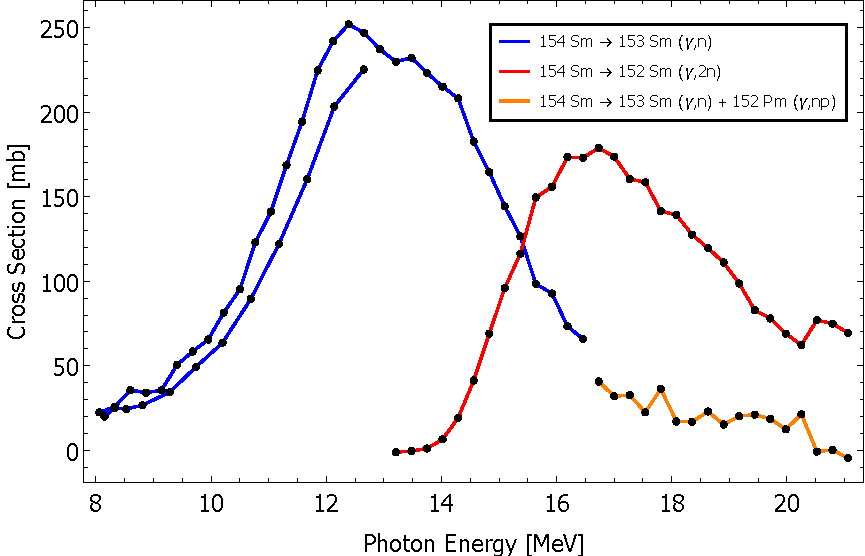
\includegraphics[width=0.8\textwidth]{Figures/DIANA_Inverse_Compton_Source_Design/Sm154Landscape.pdf}
\caption{Reaction cross section against incident photon energy for the $^{154}\mathrm{Sm} \left(\gamma,n\right)$ reaction of interest (blue, higher data \cite{carlos1974giant}, lower data \cite{filipescu2014photoneutron}), and the potentially disruptive reactions $^{154}\mathrm{Sm} \left(\gamma,2n\right)$ (red \cite{carlos1974giant}) and $^{154}\mathrm{Sm} \left(\gamma,n\right) + \left(\gamma,np\right)$ (orange \cite{carlos1974giant}). Data for other reactions photonuclear reactions involving $^{154}\mathrm{Sm}$ was unavailable. Data acquired from the EXFOR database \cite{zerkin2018experimental}. }
\label{fig:154Sm_cross_section_photon_energy}
\end{figure}

In Fig.~\ref{fig:154Sm_cross_section_photon_energy}, two measurements of the $^{154}\mathrm{Sm}\left(\gamma,n\right)$ cross section are made by Filipescu et al \cite{filipescu2014photoneutron}, using the NewSUBARU $\gamma$-ray source \cite{utsunomiya2015gamma}, and Carlos et al \cite{carlos1974giant}, where monochromatic $\gamma$-rays were generated using in-flight positron annihilation \cite{miller1960monochromatic}.

The in-flight positron annihilation used by Carlos et al involves a positron beam incident upon a target at the end of a 60~\si{\mega\electronvolt} linac at Saclay \cite{audit1970etude}. In-flight positron annihilation methods produce both a narrowband radiation spectral line resulting from positron--electron annihilations in the target as well as the typical bremsstrahlung radiation spectrum; the two can't be disentangled, but the ratio of the signal of the positron annihilation to the bremsstrahlung spectrum can typically be maximised through use of a small collimation angle resulting in collimated fluxes of $1.5\times10^{3}$~ph/\si{\second} and FWHM bandwidths of $\sim 12$\% for the upgraded Saclay source \cite{veyssiere1979quasi}.

Comparing the Saclay positron source with the NewSUBARU ICS source, as shown in Table~\ref{tab:gammaray_ICS_comparison}, the flux for the NewSUBARU ICS source would be $\mathcal{F}=3\times 10^{7}$~ph/\si{\second} -- higher than the upgraded Saclay positron annihilation source \cite{veyssiere1979quasi}. Therefore the NewSUBARU ICS source measurement has a better signal-to-noise ratio and the FWHM bandwidth of NewSUBARU is 1-2\%, a factor of 6 improvement on the Saclay upgraded source. Therefore, the NewSUBARU $^{153}\mathrm{Sm}\left(\gamma,n\right)$ measurement offers superior precision and is considered within the rest of this investigation.  

Fig.~\ref{fig:154Sm_cross_section_photon_energy} shows that the known competing processes for a mono-isotopic $^{154}\mathrm{Sm}$ can be avoided below 13.21~\si{\mega\electronvolt} as this is the threshold for the $^{154}\mathrm{Sm}\left(\gamma,2n\right)$ photonuclear reaction \cite{carlos1974giant}. However, some of the data presented by Carlos et al \cite{carlos1974giant} for the disruptive processes has negative cross sections, which is unphysical. The peak cross sections for the desired $^{154}\mathrm{Sm}\left(\gamma,n\right)$ reaction are $\sigma_{\mathrm{reac}} = 252.1$~\si{\milli\barn} at $E_{\gamma} = 12.39$~\si{\mega\electronvolt} (Carlos et al \cite{carlos1974giant}) and $\sigma_{\mathrm{reac}} = 225.3$~\si{\milli\barn} at $E_{\gamma} = 12.65$~\si{\mega\electronvolt} (Filipescu et al \cite{filipescu2014photoneutron}). Therefore, we select the Filipescu et al \cite{filipescu2014photoneutron} data based on the reasoning above. Tuning the DIANA ICS source to $E_{\gamma}=12.65$~\si{\mega\electronvolt}, the scattered photon energy  corresponding to the peak cross section ($\sigma_{\mathrm{reac}}=225.5$~\si{\milli\barn}), the maximum specific activity photonuclear production of $^{153}\mathrm{Sm}$ is possible.

By using the flux density at the target for a tuned DIANA ICS source (see Table~\ref{tab:example_isotope_cross_section_flux_density}) along with the cross section data, the specific activity (Eq.~\ref{eq:specific_activity}) of $^{153}\mathrm{Sm}$ production using DIANA can be predicted. An assumption is made all of the 0.5\% \textit{rms} bandwidth acts at the peak cross section (which is an overestimation) but is justified as inspection of Fig.~\ref{fig:DIANA_spectra} shows the energy variation here would be of the order $\Delta E_{\gamma}\sim0.5$~\si{\mega\electronvolt} and the peak cross section in Fig.~\ref{fig:154Sm_cross_section_photon_energy} varies minimally for this scattered photon energy range. 

The peak cross section assumption results in a small overestimation of the produced specific activity, however this test case is poorly optimised for maximum specific activity production, so higher specific activities may be possible. For example, a larger bandwidth may result in a larger photon flux density in the region where the ($\gamma,n$) reaction cross section is still near peak values. Optimisation of $\gamma$-ray ICS sources for photonuclear medical isotope production is a topic for further work. The specific activity as a function of irradiation time (Eq.~\ref{eq:specific_activity}) for $^{153}\mathrm{Sm}$ is shown in Fig.~\ref{fig:153Sm_specific_activity}.
\begin{figure}[!h]
\centering
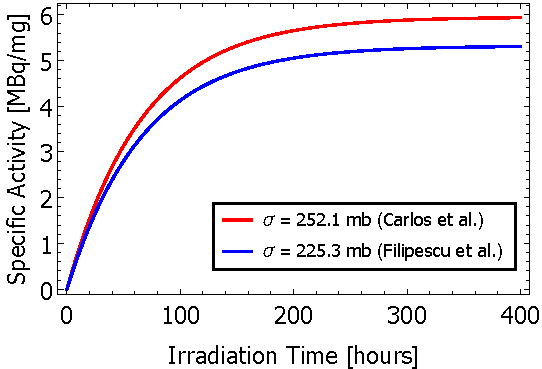
\includegraphics[width=0.6\textwidth]{Figures/DIANA_Inverse_Compton_Source_Design/154Sm_specific_activity.pdf}
\caption{Estimated specific activity of the produced $^{153}\mathrm{Sm}$ as a function of irradiation time using the collimated flux of the DIANA ICS source operating in a 0.5\% \textit{rms} bandwidth at the peak photoneutron reaction cross section, as measured by Carlos et al \cite{carlos1974giant} (red) and Filipescu et al \cite{filipescu2014photoneutron} (blue).}
\label{fig:153Sm_specific_activity}
\end{figure}

As shown in Fig.~\ref{fig:153Sm_specific_activity}, within $\sim 10$ days of irradiation the specific activity of the sample reaches a maximum of 61.07~\si{\mega\becquerel}/\si{\milli\gram} (Filipescu et al \cite{filipescu2014photoneutron}). However, if there are irradiation time constraints, as is likely, the radioisotopic sample will not achieve the saturated specific activity (Eq.~\ref{eq:sat_specific_activity}) -- where activity is not increased by further irradiation. The saturated specific activity of the photonuclear production method is far below the highest specific activity of $A/m=220$~\si{\giga\becquerel}/\si{\milli\gram} achieved at MURR \cite{ma1996production}; however, typically Quadramet is produced for clinical applications with a specific activity of 16--65~\si{\giga\becquerel}/\si{\milli\gram} \cite{ema2015quadramet} -- a factor 1000 below estimated specific activity production at the DIANA $\gamma$-ray ICS source. Photonuclear production is advantageous as no $^{154}\mathrm{Eu}$ is produced within the photonuclear route, so samarium lexidronam pentasodium may be produced with a longer shelf life.
 
With optical cavities on the 100's~\si{\kilo\watt} scale becoming widely available \cite{eggl2016munich,liu2018optical}, the possibility of improving interaction dynamics using crab cavities \cite{variola2011luminosity,koshiba2018luminosity} and the increasing the average power frontier of ERLs, the flux density available from $\gamma$-ray ICS sources could be increased and photonuclear production of radioisotopes would consequently become more feasible. There is also the additional possibility of increasing specific activity by targeting nuclear resonances for improved photoneutron reaction cross sections \cite{habs2011production}, though this hasn't been investigated within this work. However, proof-of-principle experiments involving photoneutron production of $^{153}\mathrm{Sm}$ could be conducted at the DIANA $\gamma$-ray ICS source, and optimisation of photonuclear production of radioisotopes is a possible topic for future work. Furthermore, $^{153}\mathrm{Sm}$ is selected as a single example, many more radioisotopes, for example terbium-155, have been identified as isotopes of interest for photonuclear production during this work. Exploration of these other isotopes may show more suitable candiates for photonuclear production.      

\section{Summary}

The design of a series of ICS sources for the conceptual DIANA ERL has shown the feasibility of a multi-colour $\gamma$-ray source producing high energy scattered photons $E_{\gamma}<20.11$~\si{\mega\electronvolt} and a high flux $\mathcal{F}<6.08\times 10^{10}$~ph/\si{\second}. Using the novel non-round beam optimisations from Chapter~\ref{Optimisation_and_Characterisation_of_Inverse_Compton Scattering_Spectra}, a maximal collimated flux $\mathcal{F}_{\mathrm{col}}=1.30\times 10^{9}$~ph/\si{\second} in a narrow 0.5\% \textit{rms} bandwdith has been proposed as a potential working point for the DIANA ICS source. The anticipated flux and bandwidth for the DIANA ICS source is comparable to that of the flagship ELI-NP-VEGA \cite{elinp2019vega,tanaka2020current} $\gamma$-ray source and exceeds that of the current highest demonstration at HI$\gamma$S \cite{weller2009research}, as shown in Section~\ref{sec:gamma_ICS_comparison}, with a readily achievable parameter set.

High flux quasi-monochromatic radiation production ($\Delta E_{\gamma}/E_{\gamma} < 1$\%) has been shown to be feasible for ICS sources, whereas this is not possible at other competing $\gamma$-ray sources such as those utilising bremsstrahlung production. Consequently, applications such as nuclear resonance fluorescence, transmutation of nuclear waste and medical isotope production are enabled. These applications have been investigated, and it can be concluded that preliminary experiments in each application would be feasible using the DIANA ICS source with the current design.

\end{document}